\documentclass[11pt,a4paper]{article}

% French
\usepackage[utf8x]{inputenc}
\usepackage[frenchb]{babel}
\usepackage[T1]{fontenc}
\usepackage{lmodern}
\usepackage{url}

% Math symbols
\usepackage{amsmath}
\usepackage{amssymb}
\usepackage{amsthm}
\usepackage{subfigure} %Allows to have several figures on the same line.
\usepackage{hyperref} %Allows to make references (\ref{}), pdf links are now clickable.
\usepackage{fmtcount} %Allows to use counters
\usepackage{fourier-orns} % Allows to display the \danger symbol
\usepackage{here} % Allows to place a figure where we want

\usepackage{makeidx} %Allows to create an index
\usepackage{enumerate} %Used where??
\makeindex
\usepackage[totoc]{idxlayout} %Allows to add the index in the table of contents

% Theorem and definitions
\theoremstyle{definition}
\newtheorem{mydef}{Définition}[subsection]
\newtheorem{mynota}[mydef]{Notation}
\newtheorem{myprop}[mydef]{Propriétés}
\newtheorem{myrem}[mydef]{Remarque}
\newtheorem{myform}[mydef]{Formules}
\newtheorem{mycorr}[mydef]{Corrolaire}
\newtheorem{mytheo}[mydef]{Théorème}
\newtheorem{mylem}[mydef]{Lemme}
\newtheorem{myexem}[mydef]{Exemple}
\newtheorem{myalgo}[mydef]{Algorithme}

\usepackage{algorithm}
\usepackage{algorithmic}

\newcommand{\bigoh}{\mathcal{O}}

\usepackage{tkz-graph}
\usepackage{tikz}
\usetikzlibrary{arrows,matrix,decorations.pathreplacing,positioning,chains,fit,shapes,calc} %Voir 1.3.8

\definecolor{mygreen}{rgb}{0,0.6,0}
\definecolor{mygray}{rgb}{0.5,0.5,0.5}
\definecolor{mymauve}{rgb}{0.58,0,0.82}

\tikzstyle{vertex}=[circle,fill=gray!50,minimum size=15pt,inner sep=0pt]
\tikzstyle{visited}=[circle,fill=green!25,minimum size=15pt,inner sep=0pt]
\tikzstyle{unvisited}=[circle,fill=blue!25,minimum size=15pt,inner sep=0pt]

\newcommand{\W}{\ {\color{red} \textbf{!!}} \ }

% Flots
\newcommand{\flotmax}{f_\mathrm{max}}
\DeclareMathOperator{\fnet}{f_\mathrm{net}}
\DeclareMathOperator{\coupe}{capacité}
\DeclareMathOperator{\coupemin}{\mathrm{coupe}_\mathrm{min}}
\DeclareMathOperator{\degin}{\deg_\mathrm{in}}
\DeclareMathOperator{\degout}{\deg_\mathrm{out}}
\DeclareMathOperator{\valeur}{valeur}
\DeclareMathOperator{\voisin}{Voisin}


\usepackage{verbatim} % for comment

\usepackage[framemethod=tikz]{mdframed}
%\usepackage{tikzpagenodes}
\usepackage{hyperref} %Allows to make references (\ref{}), pdf links are now clickable.
\usetikzlibrary{calc, arrows}

% greyarrow has much better handling of page breaks, see the link on stackoverflow for more info
\def\SolStyle{greyarrow}
\ifthenelse{\isundefined{\SolStyle}}{\def\SolStyle{greyarrow}}{}
\ifthenelse{\equal{\SolStyle}{greyarrow}}
{
  %http://tex.stackexchange.com/questions/50877/excursus-environment-using-mdframed-issue-with-page-breaks
\tikzset{
   excursus arrow/.style={%
    line width=2pt,
    draw=gray!40,
    rounded corners=2ex,
   },
   excursus head/.style={
    fill=white,
    font=\bfseries\sffamily,
    text=gray!80,
    anchor=base west,
   },
}

\mdfdefinestyle{mysquare}{%
  singleextra={%
   \path let \p1=(P), \p2=(O) in (\x2,\y1) coordinate (Q);%
   \path let \p1=(Q), \p2=(O) in (\x1,{(\y1-\y2)/2}) coordinate (M);%
   \path [excursus arrow, round cap-to]%
   ($(O)+(5em,0ex)$) -| (M) |- %
   ($(Q)+(12em,0ex)$) .. controls +(0:16em) and +(185:6em) .. %
   ++(23em,2ex);%
   \node [excursus head] at ($(Q)+(2.5em,-0.75pt)$) {Solution};},
  firstextra={%
   \path let \p1=(P), \p2=(O) in (\x2,\y1) coordinate (Q);
   \path [excursus arrow,-to]
   (O) |- %
   ($(Q)+(12em,0ex)$) .. controls +(0:16em) and +(185:6em) .. %
    ++(23em,2ex);
   \node [excursus head] at ($(Q)+(2.5em,-2pt)$) {Solution};
  },
  secondextra={%
   \path let \p1=(P), \p2=(O) in (\x2,\y1) coordinate (Q);
   \path [excursus arrow,round cap-]
   ($(O)+(5em,0ex)$) -| (Q);
  },
  middleextra={%
   \path let \p1=(P), \p2=(O) in (\x2,\y1) coordinate (Q);
   \path [excursus arrow](O) -- (Q);
 },
 middlelinewidth=2.5em,middlelinecolor=white,
 hidealllines=true,topline=true,
 innertopmargin=0.5ex,
 innerbottommargin=2.5ex,
 innerrightmargin=2pt,
 innerleftmargin=2ex,
 skipabove=0.87\baselineskip,
 skipbelow=0.62\baselineskip,
}

}
{
  %http://tex.stackexchange.com/questions/107191/indented-box-that-split-in-multiple-pages
\mdfdefinestyle{mysquare}{%
  leftmargin=0pt,
  rightmargin={\dimexpr4pt+2ex\relax},
  innertopmargin=2\baselineskip,
  skipabove={\dimexpr0.5\baselineskip+\topskip\relax},
  skipbelow={\dimexpr0.5\baselineskip+\topskip\relax},
  singleextra={% Single extra applies when it fits in a single page
  \path let \p1=(P), \p2=(O)
    in node[font=\bfseries] at ([yshift=-2ex]0.5*\x1-\x2,\y1) {Solution};
  \fill[black] ([xshift=2pt,yshift=2pt]P) rectangle ++(1ex,1ex);
  \fill[black] ([xshift=-2pt,yshift=-2pt]O) rectangle ++(-1ex,-1ex);
  \fill[black] ([xshift=-2pt,yshift=2pt]O|-P) rectangle ++(-1ex,1ex);
  \fill[black] ([xshift=2pt,yshift=-2pt]O-|P) rectangle ++(1ex,-1ex);
  },
  firstextra={% First extra applies on the first page when it doesn't fit in one page
  \path let \p1=(P), \p2=(O)
    in node[font=\bfseries] at ([yshift=-2ex]0.5*\x1-\x2,\y1) {Solution};
  \fill[fill=black] ([xshift=2pt,yshift=2pt]P) rectangle ++(1ex,1ex);
  \fill[black] ([xshift=-2pt,yshift=2pt]O|-P) rectangle ++(-1ex,1ex);
  },
  secondextra={% First extra applies on the last page when it doesn't fit in one page
  \fill[fill=black] ([xshift=2pt,yshift=-2pt]O-|P) rectangle ++(1ex,-1ex);
  \fill[black] ([xshift=-2pt,yshift=-2pt]O) rectangle ++(-1ex,-1ex);
  }
}

}


\ifthenelse{\isundefined{\Sol}}{\def\Sol{true}}{}
\ifthenelse{\equal{\Sol}{false}}
{
  \newenvironment{solution}{\expandafter\comment}{\expandafter\endcomment}
}
{
  \newmdenv[style=mysquare]{solution}
}

\newcommand{\nosolution}
{Cet exercice ne contient pas encore de solution.
Vous êtes invité à nous en soumettre une à l'adresse suivante
\begin{center}
\url{https://github.com/blegat/LINMA1691}
\end{center}
ou par mail.}

\parindent0mm

\setlength{\textwidth}{15cm}
\setlength{\oddsidemargin}{0.50cm}
\setlength{\textheight}{8.7in}
\setlength{\topmargin}{-0.5in}

\newcommand{\R}{{\mbox{\bf R}}}

\title{INMA1691 - Théorie et Algorithmique des Graphes : Exercices}
\author{
  Robin Ballarini
  \and Annelies Bauwens
  \and Gilles Bertrand
  \and Armand Bosquillon de Jenlis
  \and Romain Capron
  \and Arnaud Cerckel
  \and Charlotte Cirriez
  \and Simon Claessens
  \and Gaëtan Collart
  \and Matthieu Constant
  \and Xavier Crochet
  \and Gatien De Callataÿ
  \and François Dederichs
  \and Sébastien De Fauw
  \and François Delcourt
  \and Arnaud de Lhoneux
  \and Martin De Neuville
  \and Guillaume Derval
  \and Alexandre de Touzalin
  \and Gauthier Feuillen
  \and Florentin Goyens
  \and Arnaud Jacques
  \and Antoine Hilhorst
  \and Benoît Legat
  \and Arthur Losseau
  \and Alexis Pierret
  \and Thérèse Plissart
  \and François Raucent
  \and Félicien Schiltz
  \and Mélanie Sedda
  \and Benoît Sluysmans
  \and Nicolas Stevens
  \and Harold Taeter
  \and Kim Van Den Eeckhaut
  \and Geoffroy Vanderreydt
  \and Antoine Van Malleghem
  \and Nicolas Vico}


\begin{document}
%%%%%%%%%%%%%%%%%%%%%%%%%%%%%%%%%%%%%%%%%%%%%%%%%%%%%%%%%%%%%%%
%%%%%%%%%%%%%%%%%%%%%%%% PAGE DE GARDE %%%%%%%%%%%%%%%%%%%%%%%%
%%%%%%%%%%%%%%%%%%%%%%%%%%%%%%%%%%%%%%%%%%%%%%%%%%%%%%%%%%%%%%%
\pagenumbering{gobble}% Remove page numbers
\maketitle
\begin{center}
  \textit{Basé sur les séances de TP données par
  Adeline Decuyper et Romain Hollanders}\\
  \includegraphics[width=100pt]{../img/logo}\\
  \textbf{Code source et bug tracker}\\
  \url{https://github.com/blegat/LINMA1691}
\end{center}
\newpage
\clearpage

%%%%%%%%%%%%%%%%%%%%%%%%%%%%%%%%%%%%%%%%%%%%%%%%%%%%%%%%%%%%%%%
%%%%%%%%%%%%%%%%%%%%%%% Table Of Contents %%%%%%%%%%%%%%%%%%%%%
%%%%%%%%%%%%%%%%%%%%%%%%%%%%%%%%%%%%%%%%%%%%%%%%%%%%%%%%%%%%%%%
\pagenumbering{arabic}% Arabic page numbers (and reset to 1)
\tableofcontents

\section{Graphes connexes, eulériens et bipartis }
\subsection{Graphes}

\index{graphe}
\begin{mydef}
  \label{def:graph}
  Un \emph{graphe} est un triplet ($V$, $E$, $\varphi$), où :
  \begin{itemize}
    \item $V$ est un ensemble dont les éléments sont appelés sommets ou noeuds;
    \item $E$ est un ensemble dont les éléments sont appelés arêtes;
    \item $\varphi$ est une fonction, dîte fonction d'incidence, qui associe à chaque arête un sommet ou une \emph{paire} de sommets.
  \end{itemize}
\end{mydef}

\index{sommets adjacents}
\begin{mydef}
  Deux sommets incidents à la même arête sont dits \emph{adjacents}.
\end{mydef}

\index{boucle}
\begin{mydef}
  Une arête incidente à un seul sommet est une \emph{boucle}.
\end{mydef}

\index{degré}
\begin{mydef}
  Le \emph{degré} d'un sommet est le nombre d'arêtes incidentes à celui-ci.
\end{mydef}

\index{graphe!sous-graphe}
\begin{mydef}

  Un \emph{sous-graphe du graphe} ($V$, $E$, $\varphi$) est un graphe ($V'$, $E'$, $\varphi'$) avec :
  \begin{itemize}
    \item $V' \subseteq V$ ;
    \item $E' \subseteq E$ ;
    \item $\varphi'$ est la restriction de $\varphi$ à $E'$.
  \end{itemize}

\end{mydef}

\index{isomorphisme}
\subsection{Isomorphisme de Graphes}
\begin{mydef}
  Deux graphes ($V$, $E$, $\varphi$) et ($V'$, $E'$, $\varphi'$) sont dits \emph{isomorphes} s'il existe des bijections $f:V \to V'$ et $g:E \to E'$ telles que :
  \begin{center}
    $\varphi(e) = \{u, v\}$ ssi $\varphi(g(e)) = \{f(u), f(v)\}$.
  \end{center}
  Deux graphes sont isomorphes s'il y a une bijection entre les noeuds et les arêtes.
\end{mydef}

\begin{myexem}
  Voici deux exemples d'isomorphisme du même graphe :
    \begin{figure} [!h]
      \centering
	    \subfigure[]
    	{
    	  \begin{tikzpicture}[scale = 0.75]
          \node[draw, circle] at ( 0, 1.5)  (1) {1};
          \node[draw, circle] at ( 2, 0  )  (2) {2};
          \node[draw, circle] at ( 1,-1.5)  (3) {3};
          \node[draw, circle] at (-1,-1.5)  (4) {4};
          \node[draw, circle] at (-2, 0  )  (5) {5};

          \draw[-] (1) edge [bend left] node[anchor = south] {a} (2);
          \draw[-] (2) edge [bend left] node[anchor = west]  {b} (3);
          \draw[-] (3) edge [bend left] node[anchor = north] {c} (4);
          \draw[-] (4) edge [bend left] node[anchor = east]  {d} (5);
          \draw[-] (5) edge [bend left] node[anchor = east]  {e} (1);
        \end{tikzpicture}
      }
      % Cette ligne de commentaire semble être nécessaire pour que les figures soient affichées sur une ligne
      \subfigure[]
      {
        \begin{tikzpicture}[scale = 0.75]
          \node[draw, circle] at ( 0, 1.5)  (1) {$1'$};
          \node[draw, circle] at ( 2, 0.5)  (2) {$2'$};
          \node[draw, circle] at ( 1,-1.5)  (3) {$3'$};
          \node[draw, circle] at (-1,-1.5)  (4) {$4'$};
          \node[draw, circle] at (-2, 0.5)  (5) {$5'$};

          \draw[-] (1) edge [bend left] node[pos=0.05, anchor = west] {$a'$} (3);
          \draw[-] (2) edge node[anchor = north] {$b'$} (5);
          \draw[-] (2) edge node[pos=0.5, anchor = west] {$c'$} (4);
          \draw[-] (3) edge node[pos=0.5, anchor = east] {$d'$} (5);
          \draw[-] (1) edge [bend right] node[pos=0.05, anchor = east] {$e'$} (4);

        \end{tikzpicture}
      }
      % Cette ligne de commentaire semble être nécessaire pour que les figures soient affichées sur une ligne
      \subfigure[]
      {
        \begin{tikzpicture}[scale = 0.75]
          \node[draw, circle] at ( 0, 1.5)  (1) {$1'$};
          \node[draw, circle] at ( 2, 0  )  (4) {$4'$};
          \node[draw, circle] at ( 1,-1.5)  (2) {$2'$};
          \node[draw, circle] at (-1,-1.5)  (5) {$5'$};
          \node[draw, circle] at (-2, 0  )  (3) {$3'$};

          \draw[-] (1) edge [bend left] node[anchor = south] {$e'$} (4);
          \draw[-] (4) edge [bend left] node[anchor = west]  {$c'$} (2);
          \draw[-] (2) edge [bend left] node[anchor = north] {$b'$} (5);
          \draw[-] (5) edge [bend left] node[anchor = east]  {$d'$} (3);
          \draw[-] (3) edge [bend left] node[anchor = east]  {$a'$} (1);
        \end{tikzpicture}
      }
    \end{figure}
    Notons que les graphes \emph{b} et \emph{c} sont les mêmes, leurs noeuds ont simplement été réordonnés.\\
    L'isomorphisme entre \emph{a} et les deux autres est donné par : \\

    \begin{tabular}{lll}
      $f(1)=1'$ & $g(a)=e'$ \\
      $f(2)=4'$ & $g(b)=c'$ & $\varphi(a) = \{1, 2\}$\\
      $f(3)=2'$ & $g(c)=b'$ & $\varphi'(a') = \{1', 3'\}$\\
      $f(4)=5'$ & $g(d)=d'$ & $\varphi'(g(a)) = \{f(1), f(2)\}$\\
      $f(5)=3'$ & $g(e)=a'$ \\
    \end{tabular}
    \newline
    \newline
    \noindent
    Notons aussi que plusieurs résultats sont possibles :
    \begin{figure}[!h]
      \centering
      \subfigure[]
      {
        \begin{tikzpicture}[scale = 0.75]
          \node[draw, circle] at ( 0, 1.5)  (1) {1};
          \node[draw, circle] at ( 2, 0  )  (2) {2};
          \node[draw, circle] at ( 1,-1.5)  (3) {3};
          \node[draw, circle] at (-1,-1.5)  (4) {4};
          \node[draw, circle] at (-2, 0  )  (5) {5};

          \draw[-] (1) edge [bend left] node[anchor = south] {a} (2);
          \draw[-] (2) edge [bend left] node[anchor = west]  {b} (3);
          \draw[-] (3) edge [bend left] node[anchor = north] {c} (4);
          \draw[-] (4) edge [bend left] node[anchor = east]  {d} (5);
          \draw[-] (5) edge [bend left] node[anchor = east]  {e} (1);
        \end{tikzpicture}
      }
      % Cette ligne de commentaire semble être nécessaire pour que les figures soient affichées sur une ligne
      \subfigure[]
      {
        \begin{tikzpicture}[scale = 0.75]
          \node[draw, circle] at ( 0, 1.5)  (1) {$1'$};
          \node[draw, circle] at ( 2, 0.5)  (2) {$2'$};
          \node[draw, circle] at ( 1,-1.5)  (3) {$3'$};
          \node[draw, circle] at (-1,-1.5)  (4) {$4'$};
          \node[draw, circle] at (-2, 0.5)  (5) {$5'$};

          \draw[-] (1) edge [bend left] node[pos=0.05, anchor = west] {$a'$} (3);
          \draw[-] (2) edge node[anchor = north] {$d'$} (5);
          \draw[-] (2) edge node[pos=0.5, anchor = west] {$c'$} (4);
          \draw[-] (3) edge node[pos=0.5, anchor = east] {$b'$} (5);
          \draw[-] (1) edge [bend right] node[pos=0.05, anchor = east] {$e'$} (4);
        \end{tikzpicture}
      }
      \subfigure[]
      {
        \begin{tikzpicture}[scale = 0.75]
          \node[draw, circle] at ( 0, 1.5)  (1) {$1'$};
          \node[draw, circle] at ( 2, 0  )  (3) {$3'$};
          \node[draw, circle] at ( 1,-1.5)  (5) {$5'$};
          \node[draw, circle] at (-1,-1.5)  (2) {$2'$};
          \node[draw, circle] at (-2, 0  )  (4) {$4'$};

          \draw[-] (1) edge [bend left] node[anchor = south] {$a'$} (3);
          \draw[-] (3) edge [bend left] node[anchor = west]  {$b'$} (5);
          \draw[-] (5) edge [bend left] node[anchor = north] {$d'$} (2);
          \draw[-] (2) edge [bend left] node[anchor = east]  {$c'$} (4);
          \draw[-] (4) edge [bend left] node[anchor = east]  {$e'$} (1);
        \end{tikzpicture}
      }
    \end{figure}

    \begin{tabular}{lll}
      $f(1)=1'$ & $g(a)=a'$ \\
      $f(2)=3'$ & $g(b)=b'$ \\
      $f(3)=5'$ & $g(c)=d'$ \\
      $f(4)=2'$ & $g(d)=c'$ \\
      $f(5)=4'$ & $g(e)=e'$ \\
    \end{tabular}
    \newline
    \newline
    Les six graphes de cet exemple sont isomorphes entre eux.
\end{myexem}

\subsection{Parcours eulérien}
\index{parcours}
\begin{mydef}
  Un \emph{parcours} est fermé si $v_0 = v_n$.
\end{mydef}

\index{chemin}
\begin{mydef}
  Un \emph{chemin} est un parcours dont tous les sommets sont distincts.
\end{mydef}

\index{cycle}
\begin{mydef}
  Un \emph{cycle} est un parcours fermé dont tous les sommets d'origine et intérieurs sont tous distincts.
\end{mydef}

\index{graphe!graphe connexe}
\begin{mydef}
  Un \emph{graphe} est \emph{connexe} si pour chaque pair de points il existe un parcours qui les relie. Les \emph{composantes connexes} d'un graphe sont ses sous-graphes connexes maximaux.
\end{mydef}

\index{parcours!parcours eulérien}
\index{graphe!graphe eulérien}
\begin{mydef}
  Un \emph{parcours} est \emph{eulérien} s'il visite chaque arête une et une seule fois. Un \emph{graphe} est \emph{eulérien} s'il existe un parcours eulérien fermé.
\end{mydef}

\begin{mytheo} [Théorème d'Euler]
  Un graphe connexe est eulérien ssi tous les sommets sont de degré pair.
  \begin{proof}
    \noindent
    \newline
    \fbox{$\Longrightarrow$}
    \newline
    Chaque arête incidente à un noeud $x$ est utilisé par le parcours eulérien:
    \begin{itemize}
      \item soit pour entrer dans $x$;
      \item soit pour en sortir.
    \end{itemize}
    A chaque arête entrante correspond une arête sortante (celle qui suit dans le parcours sauf pour la dernière et la première).\\
    Donc, il y a une bijection entre les arêtes entrantes et les arêtes sortantes.\\
    $\longrightarrow$ degré pair \\

    \noindent
    \fbox{$\Longleftarrow$}
    \newline
    On va construire un parcours eulérien :
    \begin{enumerate}
      \item On part d'un noeud arbitraire $x_0$.
      \item On prend une arête incidente à $x_0$, on arrive à un nouveau noeud.
      \item Par parité, il y a au moins une arête non utilisée, on la prend, etc... Quand il n'y a plus d'arête disponible, on est forcément arrivé à $x_0$.
    \end{enumerate}
    \begin{center}
      \begin{tikzpicture}[scale = 0.75]
        \node[draw, circle] at (-3, 0  )  (1)  {$x_0$};
        \node[draw, circle] at (-2, 1.5)  (2)  {};
        \node[draw, circle] at (-2,-1.5)  (3)  {};
        \node[draw, circle] at (-1, 0  )  (4)  {};
        \node[draw, circle] at ( 0, 1.5)  (5)  {};
        \node[draw, circle] at ( 0,-1.5)  (6)  {};
        \node[draw, circle] at ( 1, 0  )  (7)  {$x_1$};
        \node[draw, circle] at ( 2, 1.5)  (8)  {};
        \node[draw, circle] at ( 2,-1.5)  (9)  {};
        \node[draw, circle] at ( 3, 0  )  (10) {};

        \draw[-] (1) edge node {} (2);
        \draw[dotted] (1) edge node {} (3);
        \draw[-] (2) edge node {} (4);
        \draw[-] (3) edge node {} (4);
        \draw[-] (4) edge node {} (5);
        \draw[-] (4) edge node {} (6);
        \draw[-] (5) edge node {} (7);
        \draw[-] (6) edge node {} (7);
        \draw[-] (7) edge node {} (8);
        \draw[-] (7) edge node {} (9);
        \draw[-] (8) edge node {} (10);
        \draw[-] (9) edge node {} (10);
      \end{tikzpicture}
    \end{center}
    Pour tout autre noeud y, en arrivant à y, on a utilisé un nombre impair d'arêtes incidentes à y. On a un parcours fermé :
    \begin{itemize}
      \item Si toutes les arêtes incidentes aux x noeuds traversés par ce parcours sont utilisées, alors ce parcours est eulérien;
      \item Sinon, il y a $x_1 \in$ parcours avec au moins une arête non exploitée.
    \end{itemize}
    \begin{center}
      \begin{tikzpicture}[scale = 0.75]
        \node[draw, circle] at (-4, 0  )  (1)  {};
        \node[draw, circle] at (-4,-1.5)  (2)  {};
        \node[draw, circle] at (-2, 0  )  (3)  {$x_0$};
        \node[draw, circle] at (-2,-1.5)  (4)  {};
        \node[draw, circle] at (-2, 1.5)  (5)  {};
        \node[draw, circle] at ( 0, 1.5)  (6)  {};
        \node[draw, circle] at ( 0, 0  )  (7)  {$x_1$};
        \node[draw, circle] at ( 0,-1.5)  (8)  {};
        \node[draw, circle] at ( 2,-1.5)  (9)  {};
        \node[draw, circle] at ( 2, 0  )  (10) {};

        \draw[-] (1) edge node {} (2);
        \draw[-] (1) edge node {} (3);
        \draw[-] (2) edge node {} (4);
        \draw[-] (3) edge node {} (4);
        \draw[-] (3) edge node {} (5);
        \draw[-] (3) edge node {} (7);
        \draw[-] (5) edge node {} (6);
        \draw[-] (6) edge node {} (7);
        \draw[-, color=red] (7) edge node {} (8);
        \draw[-, color=red] (7) edge node {} (10);
        \draw[-, color=red] (8) edge node {} (9);
        \draw[-, color=red] (9) edge node {} (10);
      \end{tikzpicture}
    \end{center}
    On merge les deux parcours :\\
    $P_{0+1} = x_0 \rightarrow x_1 \textcolor{red}{\rightarrow} x_1 \rightarrow x_0$\\
    Et on fait ça en boucle jusqu'à avoir toutes les arêtes.
  \end{proof}
\end{mytheo}

\begin{mytheo} [Existence d’un parcours eulérien]
  Un graphe connexe possède un parcours eulérien ssi le nombre de noeuds de degré impair est zéro ou deux.
  \begin{proof}
    \noindent
    \newline
    \fbox{$\Longrightarrow$}
    \newline
    \begin{itemize}
      \item Si ce parcours eulérien est fermé, tous les degrés sont pairs;
      \item Si ce parcours eulérien est ouvert, tous les degrés sont pairs, sauf $deg(u)$ et $deg(v)$ qui sont impairs.\\
    \end{itemize}

    \noindent
    \fbox{$\Longleftarrow$}
    \newline
    \begin{itemize}
      \item Si tous les degrés sont pairs alors il existe un parcours eulérien fermé;
      \item Si deux degrés sont impairs et si on ajoute une arête $e$ entre $u$ et $v$ :\\
      $\rightarrow$ Tous les degrés sont pairs.\\
      $\rightarrow$ Il existe un parcours eulérien fermé.\\
      En retirant $e$, on obtient un parcours eulérien ouvert $u \rightarrow v$
    \end{itemize}
  \end{proof}
\end{mytheo}

\begin{mytheo} [Théorème des poignées de mains]
  La somme des degrés des noeuds d’un graphe est deux fois le nombre d’arêtes.\\
  $\sum_{v_i \in V}^{} deg(v_i) = 2|E|$
  \begin{proof}
    En utilisant la matrice d'incidence $M$ (voir \ref{in_matrix}), on peut calculer $\sum_{i,j}^{} M_{i,j}$ de deux façon différentes :\\
    \begin{tikzpicture}[decoration=brace]
      \matrix (m) [matrix of math nodes,left delimiter=[,right delimiter={]}] {
          0 & 1 & 1 & 0 & 1 & 0 \\
          1 & 1 & 0 & 1 & 0 & 1 \\
          1 & 0 & 0 & 1 & 0 & 1 \\
          0 & 0 & 1 & 0 & 1 & 0 \\
      };
      \draw[decorate,transform canvas={xshift=1.3em},thick] (m-1-6.north east) -- node[right=2pt] {$\sum_i \sum_j M_{ij} = \sum_{v_i \in V} deg(v_i)$} (m-4-6.south east);
      \draw[decorate,transform canvas={yshift=-1.7em},thick] (m-4-6.north east) -- node[below=2pt] {$\sum_i \sum_j M_{ij} = 2|E|$} (m-3-1.south west);
    \end{tikzpicture}
    \vspace*{5mm}
    \begin{center}
      $\sum_i \sum_j M_{ij} = \sum_i \sum_j M_{ij}$\\
      \vspace*{2mm}
      $2|E| = \sum_{v_i \in V} deg(v_i)$
    \end{center}
  \end{proof}
\end{mytheo}

\subsection{Représentation matricielle du graphe}
\index{matrice d'adjacence}
\begin{mydef}
  La \emph{matrice d'adjacence} est une matrice carrée $n$x$n$ dont l'élément $ij$ est le nombre d'arêtes entre les sommets $v_i$ et $v_j$.
\end{mydef}

\index{matrice d'incidence}
\begin{mydef}
  \label{in_matrix}
  La \emph{matrice d'incidence} est une matrice rectangulaire $n$x$m$ dont l'élément $ij$ est le nombre de fois que le sommet $v_i$ est incident à l'arête $e_j$.
\end{mydef}

\begin{myexem}
  \noindent
  \begin{center}
    \begin{tikzpicture}[scale = 0.75]
      \node[draw, circle] at ( 0, 4)  (1)  {$1$};
      \node[draw, circle] at ( 2, 0)  (2)  {$2$};
      \node[draw, circle] at (-2, 0)  (3)  {$3$};

      \draw[-] (1) edge [loop above] node {a} (1);
      \draw[-] (1) edge [bend left] node [anchor = north] {b} (2);
      \draw[-] (1) edge [bend right] node [anchor = north] {c} (2);
      \draw[-] (2) edge node [anchor = north] {d} (3);
      \draw[-] (1) edge node [anchor = north] {e} (3);
    \end{tikzpicture}

    $
    Matrice\ d'adjacence\ :\ A\ = \bordermatrix{~ & 1 & 2 & 3 \cr
                                                1 & 1 & 2 & 1 \cr
                                                2 & 2 & 0 & 1 \cr
                                                3 & 1 & 1 & 0 \cr}
    $

    $
    Matrice\ d'incidence\ :\ M\ = \bordermatrix{~ & a & b & c & d & e\cr
                                                1 & 2 & 1 & 1 & 0 & 1\cr
                                                2 & 0 & 1 & 1 & 1 & 0\cr
                                                3 & 0 & 0 & 0 & 1 & 1\cr}
    $
  \end{center}
  $(A^k)_{ij} =$ nombre de parcours $i \to j$ de longueur $k$.\\
  $
    A^0\ =\ I\ =  \begin{pmatrix} 1 & 0 & 0\\
                                  0 & 1 & 0\\
                                  0 & 0 & 1
                  \end{pmatrix},\
    A^1\ =\ A\ =\begin{pmatrix} 1 & 2 & 1\\
                                2 & 0 & 1\\
                                1 & 1 & 0
                \end{pmatrix},\
    A^2\ = \begin{pmatrix}  6 & 3 & 3\\
                            3 & 5 & 2\\
                            3 & 2 & 2
            \end{pmatrix}
  $
\end{myexem}

\begin{mytheo} [Matrice d’adjacence et nombre de parcours]
  Soit $A$ la matrice d'adjacence d'un graphe. Alors l'élément $ij$ de $A^k$ ($k \geq 0$) est le nombre de parcours de longueur $k$ de $v_i$ vers $v_j$.
  \begin{proof}
    Nous procédons par récurrence. Soit $A$ une matrice d'adjacence.\\
    Pour $k=0$, $A^{0}=Id$. La propriété est vérifiée par convention. Il existe un chemin de longueur 0 d'un point vers lui même. \\
    Pour $k=1$, $A^{1}=A$ représente bien le nombre de parcours de longueur 1. \\
    Supposons la propriété vérifiée pour $A^{k}$.

    Nombre de parcours de parcours de $i \to j$ de longueur $k+1 =$\\
    $= \sum_{l \in E}$ (\# parcours de $i \to l$ de longueur $k$)$.$(\# arêtes $l \to j$)\\
    $= \sum_{l \in E} A_{il}^{k}.A_{lj}$\\
    $= A_{ij}^{k+1}$
  \end{proof}
\end{mytheo}

\index{distance entre deux noeuds}
\begin{mydef}
  La \emph{distance $d(u, v)$} entre les noeuds $u$ et $v$ d'un graphe est le nombre d'arêtes minimal d'un parcours entre ces deux noeuds.
\end{mydef}

\begin{mylem}
  Si $u...u'...v'...v$ est un parcours de longeur minimale de $u$ vers $v$, alors le sous-parcours $u'...v'$ est un parcours de longeur minimale de $u'$ vers $v'$.\\
  En particulier, un parcours de longueur minimale est toujours un chemin.
  \begin{proof}
    Si ce parcours entre $u'$ et $v'$ n'était pas le plus court, on utiliserait le parcours strictement plus court pour la construction du parcours entre $u$ et $v$.
  \end{proof}
\end{mylem}

\subsection{Graphe biparti}
\index{graphe!graphe biparti}
\begin{mydef}
  Un graphe est \emph{biparti}  s'il existe une partition en deux ensembles $V_1$ et $V_2$ tels que les sommets de $V_1$ ne sont adjacents qu'à des sommets de $V_2$ et vice versa. La bipartition est $(V_1, V_2)$.
\end{mydef}

\begin{myexem}
  \noindent
  \begin{center}
    \definecolor{myblue}{RGB}{80,80,160}
    \definecolor{mygreen}{RGB}{80,160,80}

    \begin{tikzpicture}[thick,
      every node/.style={draw,circle},
      fsnode/.style={fill=myblue},
      ssnode/.style={fill=mygreen},
      every fit/.style={ellipse,draw,inner sep=-2pt,text width=2cm},
      ->,shorten >= 3pt,shorten <= 3pt
    ]

    % the vertices of U
    \begin{scope}[start chain=going below,node distance=7mm]
    \foreach \i in {1,2,...,5}
      \node[fsnode,on chain] (f\i) [label=\i] {};
    \end{scope}

    % the vertices of V
    \begin{scope}[xshift=4cm,yshift=-0.5cm,start chain=going below,node distance=7mm]
    \foreach \i in {6,7,...,9}
      \node[ssnode,on chain] (s\i) [label=\i] {};
    \end{scope}

    % the set U
    \node [myblue,fit=(f1) (f5),label=$V_1$] {};
    % the set V
    \node [mygreen,fit=(s6) (s9),label=$V_2$] {};

    % the edges
    \draw (f1) -- (s6);
    \draw (s6) -- (f2);
    \draw (f2) -- (s7);
    \draw (s7) -- (f3);
    \draw (s8) -- (f3);
    \draw (f3) -- (s9);
    \draw (s9) -- (f5);
    \draw (f5) -- (s6);
    \draw (f4) -- (s9);
    \end{tikzpicture}
  \end{center}
\end{myexem}

\begin{mytheo} [Graphes bipartis]
  Un graphe est biparti ssi tous ses cycles sont de longueur paire.
  \begin{proof}
    \noindent
    \newline
    \fbox{$\Longrightarrow$}
    \newline
    Il existe une bipartition $(V_1,V_2)$.\\
    \begin{align*}
      Cycle : & V_1, V_2, V_3, ..., V_n \Rightarrow n\ est\ pair.\\
              & \downarrow\ \ \ \downarrow\ \ \ \downarrow\ \ \ \ \ \ \ \downarrow\\
              & V_1, V_2, V_1, ..., V_2
    \end{align*}

    \noindent
    \fbox{$\Longleftarrow$}
    \newline
    Partition d'un noeud $v_0$ au hasard.\\
    $V_0\ =\ \{v|d(v,\ v_0)\ $paire$\}$\\
    $V_1\ =\ \{v|d(v,\ v_0)\ $impaire$\}$\\
    C'est une partition. Est-ce une bipartition?
    Oui, sinon on aurait par exemple une arête $uv$ dans $V_0$.

    \begin{center}
      \begin{tikzpicture}
        \node[draw, circle] at (-4, 0)  (1)  {$v_0$};
        \node[draw, circle] at (-1, 0)  (2)  {$w$};
        \node[draw, circle] at ( 2, 1)  (3)  {$u$};
        \node[draw, circle] at ( 2,-1)  (4)  {$v$};

        \draw[-] (1) edge [bend left]  node {} (2);
        \draw[-] (1) edge [bend right] node {} (2);
        \draw[-, color=red] (2) edge [bend left]  node [anchor = south, color=black] {pcc $v_0 \to u$} (3);
        \draw[-, color=red] (2) edge [bend right] node [anchor = north, color=black] {pcc $v_0 \to v$} (4);
        \draw[-, color=red] (3) edge node {} (4);
      \end{tikzpicture}
    \end{center}
    pcc : plus court chemin.\\
    Les pcc sont de longueure paire car on est dans $V_0$.\\
    $w$ est le dernier point d'intersection entre les chemins $v_0 \to u$ et $v_0 \to v$.\\
    \textcolor{red}{$\triangle$} est un cycle de longueur impaire car $w \to u$ et $w \to v$ sont paires (les deux sous-chemins de $v_0 \to w$ sont des plus court chemin de même longueur) + une arête $uv$.\\
    $lg(wuvw)\ =\ lg(v_{0}uvv_0)\ - \ 2lg(v_0w)$\\
    $impaire\ \ \ \ \ \ \ \ \ \ \ \ \ \ \ \ \ \ \ \ \ \ \ \ \ \ \ \ \ \ paire$\\
    Contradiction, si arête dans $V_1$ même raisonnement.
  \end{proof}
\end{mytheo}

\section{Séance 2}
\subsection{Parcours fermés} Dans le graphe ci-dessous, trouvez le nombre de parcours fermés de longueur $k$ contenant le point $A$.

\begin{figure}[h!]
  \begin{center}
    \begin{tikzpicture}[scale=1,looseness=1,auto,line width=.4mm]

      \path[draw=none] (-2.3,1.3) node { $A$ };

      \draw (-2, 1) -- ( 0,-1);
      \draw (-2, 1) -- ( 2,-1);
      \draw ( 0, 1) -- (-2,-1);
      \draw ( 0, 1) -- ( 2,-1);
      \draw ( 2, 1) -- (-2,-1);
      \draw ( 2, 1) -- ( 0,-1);

      \draw[fill=black] (-2,-1) circle(.12);
      \draw[fill=black] (-2, 1) circle(.12);
      \draw[fill=black] ( 0,-1) circle(.12);
      \draw[fill=black] ( 0, 1) circle(.12);
      \draw[fill=black] ( 2,-1) circle(.12);
      \draw[fill=black] ( 2, 1) circle(.12);

    \end{tikzpicture}
  \end{center}
\end{figure}

\begin{solution}
On cherche le nombre de parcours fermé partant de A de longueur $k$.
Pour cela, on utilise le théorème suivant :

$\,$

Soit $A$ la matrice d'adjacence d'un graphe. Alors l'élément $ij$
de $A^{k}$ ($k\geq0$) est le nombre de parcours de longueur $k$
de $v_{i}$ vers $v_{j}$.

$\,$

Dans notre cas, le graphe est biparti non complet et la matrice d'adjacence
est donnée par :

\[
A=\left(\begin{array}{cccccc}
0 & 0 & 0 & 0 & 1 & 1\\
0 & 0 & 0 & 1 & 0 & 1\\
0 & 0 & 0 & 1 & 1 & 0\\
0 & 1 & 1 & 0 & 0 & 0\\
1 & 0 & 1 & 0 & 0 & 0\\
1 & 1 & 0 & 0 & 0 & 0
\end{array}\right)
\]


Si $k$ est impair, la matrice d'adjacence élevée à la puissance $k$
deviendra :

\[
A^{k}=\left(\begin{array}{cc}
\begin{array}{ccc}
0 & 0 & 0\\
0 & 0 & 0\\
0 & 0 & 0
\end{array} & \left[\begin{array}{ccc}
0 & 1 & 1\\
1 & 0 & 1\\
1 & 1 & 0
\end{array}\right]^{k}\\
\left[\begin{array}{ccc}
0 & 1 & 1\\
1 & 0 & 1\\
1 & 1 & 0
\end{array}\right]^{k} & \begin{array}{ccc}
0 & 0 & 0\\
0 & 0 & 0\\
0 & 0 & 0
\end{array}
\end{array}\right)
\]


Comme on cherche des parcours fermé de A vers A, on s'intéresse uniquement
aux éléments diagonaux qui sont, dans le cas où $k$ est impair, tous
nuls. Par conséquent, le nombre de parcours fermé de longueur $k$
vaut 0.

Si $k$ est pair, la matrice d'adjacence élevée à la puissance $k$
deviendra :

\[
A^{k}=\left(\begin{array}{cc}
\left[\begin{array}{ccc}
0 & 1 & 1\\
1 & 0 & 1\\
1 & 1 & 0
\end{array}\right]^{k} & \begin{array}{ccc}
0 & 0 & 0\\
0 & 0 & 0\\
0 & 0 & 0
\end{array}\\
\begin{array}{ccc}
0 & 0 & 0\\
0 & 0 & 0\\
0 & 0 & 0
\end{array} & \left[\begin{array}{ccc}
0 & 1 & 1\\
1 & 0 & 1\\
1 & 1 & 0
\end{array}\right]^{k}
\end{array}\right)
\]


Dans ce cas, les éléments diagonaux de $A^{k}$ sont non nuls. De
plus, les sous-blocs $\left[\begin{array}{ccc}
0 & 1 & 1\\
1 & 0 & 1\\
1 & 1 & 0
\end{array}\right]^{k}$correspondent à une matrice d'adjacence élevée à la puissance $k$
d'un graphe complet. Dans la première séance d'exercice, on a démontré
une formule pour calculer une entrée de la diagonale de cette matrice
:

\[
\#\, parcours\, ferm\acute{e}\, de\, longueur\, k\, de\, A\rightarrow A=\frac{(n-1)}{n}((n-1)^{k-1}+(-1)^{k})
\]


Ici $k$ est pair, donc $(-1)^{k}=1$ et $n=3$ (sous-blocs), on obtient
:

\[
\#\, parcours\, ferm\acute{e}\, de\, longueur\, k\, de\, A\rightarrow A=\frac{2}{3}(2{}^{k-1}+1)
\]
\end{solution}

\subsection{Tracer d'un coup} Est-il possible de tracer les figures suivantes sans lever le crayon et sans passer deux fois par le même segment?

\begin{figure}[h!]
  \begin{center}
    \begin{tabular}{lcccr}
      \begin{tikzpicture}[scale=1,looseness=1,auto,line width=.4mm]

        \draw (-1, 1) -- (  0, 2);
        \draw (-1, 1) -- (-.5,.5);
        \draw (-1, 0) -- (  0,-1);
        \draw (-1, 0) -- (-.5,.5);
        \draw (-1,-1) -- (  0, 0);
        \draw (-1,-1) -- (  0,-2);
        \draw ( 1, 1) -- (  0, 2);
        \draw ( 1, 1) -- ( .5,.5);
        \draw ( 1, 0) -- (  0,-1);
        \draw ( 1, 0) -- ( .5,.5);
        \draw ( 1,-1) -- (  0, 0);
        \draw ( 1,-1) -- (  0,-2);
        \draw ( 0, 0) -- ( .5,.5);
        \draw ( 0, 0) -- (-.5,.5);
        \draw ( 0, 1) -- ( .5,.5);
        \draw ( 0, 1) -- (-.5,.5);

        \draw[fill=black] ( -1, 1) circle(.1);
        \draw[fill=black] ( -1, 0) circle(.1);
        \draw[fill=black] ( -1,-1) circle(.1);
        \draw[fill=black] (  0,-2) circle(.1);
        \draw[fill=black] (  0,-1) circle(.1);
        \draw[fill=black] (  0, 0) circle(.1);
        \draw[fill=black] (  0, 1) circle(.1);
        \draw[fill=black] (  0, 2) circle(.1);
        \draw[fill=black] (  1, 1) circle(.1);
        \draw[fill=black] (  1, 0) circle(.1);
        \draw[fill=black] (  1,-1) circle(.1);
        \draw[fill=black] (-.5,.5) circle(.1);
        \draw[fill=black] ( .5,.5) circle(.1);

      \end{tikzpicture}
      & \hspace{1cm} &
      \begin{tikzpicture}[scale=1,looseness=1,auto,line width=.4mm]

        \draw (0,0) -- (2,0);
        \draw (0,0) -- (2,2);
        \draw (0,0) -- (0,2);
        \draw (2,0) -- (2,2);
        \draw (2,0) -- (0,2);
        \draw (0,2) -- (2,2);
        \draw (0,2) -- (1,3);
        \draw (2,2) -- (1,3);

        \draw[fill=black] (0,0) circle(.1);
        \draw[fill=black] (2,0) circle(.1);
        \draw[fill=black] (2,2) circle(.1);
        \draw[fill=black] (0,2) circle(.1);
        \draw[fill=black] (1,3) circle(.1);

      \end{tikzpicture}
      & \hspace{1cm} &
      \begin{tikzpicture}[scale=1,looseness=1,auto,line width=.4mm]

        \draw (.5,0) -- (1.5,0);
        \draw (.5,0) -- (1,3);
        \draw (.5,0) -- (0,2);
        \draw (1.5,0) -- (2,2);
        \draw (1.5,0) -- (1,3);
        \draw (0,2) -- (2,2);
        \draw (0,2) -- (1,3);
        \draw (2,2) -- (1,3);

        \draw[fill=black] (.5,0) circle(.1);
        \draw[fill=black] (1.5,0) circle(.1);
        \draw[fill=black] (2,2) circle(.1);
        \draw[fill=black] (0,2) circle(.1);
        \draw[fill=black] (1,3) circle(.1);

      \end{tikzpicture}
    \end{tabular}
  \end{center}
\end{figure}

\begin{solution}
Tracer les figures sans lever le crayon et sans passer deux fois par
le même segment, revient à chercher un parcours eulérien :
\begin{itemize}
\item Tous les sommets sont de degré pair, par le théorème d'Euler on en
conclut que le graphe est eulérien. Il existe donc un parcours eulérien
fermé.
\item 2 noeuds sont de degré impair, on utilise le théorème suivant :
\end{itemize}
\begin{center}
\par Un graphe connexe possède un parcours eulérien ssi le nombre de noeuds de degré impair est zéro ou deux.

\end{center}

Il existe donc un parcours eulérien dans le premier et le deuxième.
Il y a 4 noeuds qui sont de degré impair dans le dernier, il n'existe donc pas de parcours eulérien.

\end{solution}

\subsection{Algorithme pour trouver un circuit eulérien} En vous basant sur la preuve inductive du théorème qui caractérise les graphes eulériens, décrivez un algorithme qui trouve un circuit eulérien en un temps $O(|E|)$.
\begin{solution}
Il faut utiliser la preuve du théorème d'Euler :

\begin{center}
Un graphe connexe est eulérien ssi tous les sommets sont de degré
pair
\par\end{center}

La deuxième partie de la preuve consiste en la construction d'un parcours
eulérien, cela nous donne aussi un algorithme pour trouver un parcours
eulérien.

Le principe de l’algorithme est simple:
\begin{itemize}
\item on prend un nœud non parcouru encore;
\item on prend les arêtes non parcourue encore jusqu'à revenir sur le noeud de départ;
\item on merge ce parcours avec ceux déjà trouver;
\item si il n'y a plus de nœud non exploré, on a fini. Sinon on reprend au point 1.
\end{itemize}
\end{solution}
\subsection{Séquences de de Bruijn.} Le problème suivant apparaît sous de nombreuses formes. On demande de construire la plus longue séquence circulaire de lettres d'un alphabet de $k$ lettres sans qu'aucune sous-séquence de longueur $n$ ne soit répétée.
\begin{enumerate}
  \item Donnez une borne supérieure sur la longueur de la séquence circulaire en question.
  \item Cette borne peut-elle être atteinte? Formulez cette question comme un problème de tour eulérien dans un graphe orienté. (Indice~: les sommets correspondent aux séquences de longueur $n-1$ et les arêtes aux séquences de longueur $n$.)
  \item Pour l'alphabet $\mathcal{A} = \{0, 1, 2\}$ de $k = 3$ lettres et pour $n = 3$, répondez à la question précédente en construisant la plus longue séquence circulaire.
\end{enumerate}
\begin{solution}
1. $k^{n}$ est une borne supérieure sur le nombre de sous-séquences
de longueur $n$. Puisqu'on ne peut pas les répéter, la plus longue
chaîne utilisera toutes les sous-séquences.

2.oui

3.
\end{solution}
\pagebreak
\subsection{Parcourt fermé de poid minimum} On souhaite trouver un parcours fermé de poids minimum passant au moins une fois par chaque arête du graphe suivant~:
\begin{figure}[h!]
  \begin{center}
    \begin{tikzpicture}[scale=1,auto,line width=.4mm]

      \coordinate (11++) at ( 1, 1);
      \coordinate (13++) at ( 1, 3);
      \coordinate (31++) at ( 3, 1);
      \coordinate (11+-) at ( 1,-1);
      \coordinate (13+-) at ( 1,-3);
      \coordinate (31+-) at ( 3,-1);
      \coordinate (11-+) at (-1, 1);
      \coordinate (13-+) at (-1, 3);
      \coordinate (31-+) at (-3, 1);
      \coordinate (11--) at (-1,-1);
      \coordinate (13--) at (-1,-3);
      \coordinate (31--) at (-3,-1);

      \draw (11++) -- (13++) node[midway,right] {$1$};
      \draw (11++) -- (31++) node[midway,above] {$3$};
      \draw (31++) -- (13++) node[midway,above,right] {$4$};
      \draw (11+-) -- (13+-) node[midway,right] {$1$};
      \draw (11+-) -- (31+-) node[midway,above] {$3$};
      \draw (31+-) -- (13+-) node[midway,below,right] {$4$};
      \draw (11-+) -- (13-+) node[midway,right] {$1$};
      \draw (11-+) -- (31-+) node[midway,above] {$3$};
      \draw (31-+) -- (13-+) node[midway,above,left] {$4$};
      \draw (11--) -- (13--) node[midway,right] {$1$};
      \draw (11--) -- (31--) node[midway,above] {$3$};
      \draw (31--) -- (13--) node[midway,below,left] {$4$};
      \draw (11++) -- (11+-) node[midway,right] {$2$};
      \draw (11++) -- (11-+) node[midway,above] {$2$};
      \draw (11--) -- (11+-) node[midway,above] {$2$};
      \draw (11--) -- (11-+) node[midway,right] {$2$};
      \draw (13++) -- (13-+) node[midway,above] {$7$};
      \draw (13+-) -- (13--) node[midway,above] {$7$};
      \draw (31++) -- (31+-) node[midway,right] {$1$};
      \draw (31-+) -- (31--) node[midway,right] {$1$};

      \draw[fill=black] (11++) circle(.1);
      \draw[fill=black] (13++) circle(.1);
      \draw[fill=black] (31++) circle(.1);
      \draw[fill=black] (11+-) circle(.1);
      \draw[fill=black] (13+-) circle(.1);
      \draw[fill=black] (31+-) circle(.1);
      \draw[fill=black] (11-+) circle(.1);
      \draw[fill=black] (13-+) circle(.1);
      \draw[fill=black] (31-+) circle(.1);
      \draw[fill=black] (11--) circle(.1);
      \draw[fill=black] (13--) circle(.1);
      \draw[fill=black] (31--) circle(.1);

    \end{tikzpicture}
  \end{center}
\end{figure}

\begin{solution}
Il faut trouver un parcours fermé de poids minimum passant au moins
une fois par chaque arête. Le cas idéal est celui où tous les noeuds
sont pairs car dans ce cas il existe un parcours fermé passant une
et une seule fois par chaque arête (Théorème d'Euler). Dans notre
cas, tous les noeuds sur le bord (L, E, F, G, H, I, J et K) ont degré
3. Afin de nous ramener au cas idéal (noeuds pairs), nous allons rajouter
des arêtes au graphe entre les noeuds de degré impair. Nous avons
huit noeuds de degré impair, nous les regroupons par paire de façon
à avoir le plus court chemin possible entre chaque paire de noeuds.
On a les 4 paires suivante : LE, FG, HI, KJ. Ensuite on rajoute une
arête entre chaque paire de noeud, le poids de cette nouvelle arête
correspond au poids du plus court chemin entre les noeuds incidents
à cette arête. On obtient le graphe ci-dessous :

\begin{center}
  \begin{tikzpicture}
    \node[circle] (A)[draw=black] at (1,1){A};
    \node[circle] (B)[draw=black] at (1,-1){B};
    \node[circle] (C)[draw=black] at (-1,-1){C};
    \node[circle] (D)[draw=black] at (-1,1){D};
    \node[circle] (E)[draw=black] at (1,3){E};
    \node[circle] (F)[draw=black] at (3,1){F};
    \node[circle] (G)[draw=black] at (3,-1){G};
    \node[circle] (H)[draw=black] at (1,-3){H};
    \node[circle] (I)[draw=black] at (-1,-3){I};
    \node[circle] (J)[draw=black] at (-3,-1){J};
    \node[circle] (K)[draw=black] at (-3,1){K};
    \node[circle] (L)[draw=black] at (-1,3){L};

    \path (A) edge node [right] {2} (B);
    \path (B) edge node [above] {2} (C);
    \path (C) edge node [right] {2} (D);
    \path (D) edge node [above] {2} (A);
    \path (E) edge node [above] {4} (F);
    \path (F) edge node [right] {1} (G);
    \path (G) edge node [below] {4} (H);
    \path (H) edge node [above] {7} (I);
    \path (I) edge node [below] {4} (J);
    \path (J) edge node [right] {1} (K);
    \path (K) edge node [above] {4} (L);
    \path (L) edge node [above] {7} (E);
    \path (A) edge node [right] {1} (E);
    \path (A) edge node [above] {3} (F);
    \path (B) edge node [above] {3} (G);
    \path (B) edge node [right] {1} (H);
    \path (C) edge node [right] {1} (I);
    \path (C) edge node [above] {3} (J);
    \path (D) edge node [above] {3} (K);
    \path (D) edge node [right] {1} (L);
    \draw[red,out=45,in=135] (L) to node [above] {4} (E);
    \draw[red,out=-135,in=135] (K) to node [right] {1} (J);
    \draw[red,out=-45,in=45] (F) to node [right] {1} (G);
    \draw[red,out=-45,in=-135] (I) to node [above] {4} (H);
  \end{tikzpicture}
\end{center}

A présent, nous avons un graphe composé uniquement de noeuds de degré
pair. Nous savons par le théorème d'Euler, qu'il existe un parcours
fermé passant une seule fois par chaque arête. Ce parcours est le
parcours de poids minimum passant au moins une fois par chaque arête
dans le graphe de départ, son poids correspond à la somme des poids
de chaque arête dans le nouveau graphe :

\[ 7+4+1+4+7+4+1+4+1+1+3+3+1+1+3+3+2+2+2+2+\textcolor{red}{4}+\textcolor{red}{4}+\textcolor{red}{1}+\textcolor{red}{1} = 66 \]
\end{solution}

\subsection{Chemin de coût minimum}
Dans le graphe suivant, trouvez un parcours de coût minimum du sommet $1$ au sommet $7$.
Le parcours doit traverser toutes les arêtes au moins une fois.

\begin{figure}[h!]
  \begin{center}
    \begin{tikzpicture}[scale=2,auto,line width=.4mm]

      \path (0,0) node[draw,shape=circle] (1)  {$1$};
      \path (0,1) node[draw,shape=circle] (2)  {$2$};
      \path (0,2) node[draw,shape=circle] (3)  {$3$};
      \path (1,0) node[draw,shape=circle] (6)  {$4$};
      \path (1,1) node[draw,shape=circle] (5)  {$5$};
      \path (1,2) node[draw,shape=circle] (4)  {$6$};
      \path (2,0) node[draw,shape=circle] (7)  {$7$};
      \path (2,1) node[draw,shape=circle] (8)  {$8$};
      \path (2,2) node[draw,shape=circle] (9)  {$9$};
      \path (3,0) node[draw,shape=circle] (12) {$10$};
      \path (3,1) node[draw,shape=circle] (11) {$11$};
      \path (3,2) node[draw,shape=circle] (10) {$12$};

      \draw (1)  -- (2)  node[midway,left]  {$3$};
      \draw (2)  -- (3)  node[midway,left]  {$5$};
      \draw (6)  -- (5)  node[midway,left]  {$6$};
      \draw (5)  -- (4)  node[midway,left]  {$5$};
      \draw (7)  -- (8)  node[midway,left]  {$1$};
      \draw (8)  -- (9)  node[midway,left]  {$2$};
      \draw (12) -- (11) node[midway,right] {$5$};
      \draw (11) -- (10) node[midway,right] {$2$};
      \draw (1)  -- (6)  node[midway,above] {$4$};
      \draw (2)  -- (5)  node[midway,above] {$8$};
      \draw (3)  -- (4)  node[midway,above] {$1$};
      \draw (4)  -- (9)  node[midway,above] {$3$};
      \draw (5)  -- (8)  node[midway,above] {$5$};
      \draw (6)  -- (7)  node[midway,above] {$1$};
      \draw (7)  -- (12) node[midway,above] {$3$};
      \draw (8)  -- (11) node[midway,above] {$9$};
      \draw (9)  -- (10) node[midway,above] {$7$};
      \draw (9)  -- (11) node[midway,above,right] {$1$};
      \draw (1) to[bend right] node[midway,below] {$2$} (7);

    \end{tikzpicture}
  \end{center}
\end{figure}

\begin{solution}
Le raisonnement est similaire à celui de l'exercice 5. Nous devons
trouver un chemin de coût minimum du sommet 1 au sommet 7. Le chemin
doit traverser toutes les arêtes au moins une fois. 

Le cas idéal est celui d'un parcours eulérien du sommet 1 au sommet 7 (dans ce cas
on ne passe qu'une seule fois par chaque arête). Pour avoir un parcours
eulérien, il faut que les sommets de départ et d'arrivée (sommet 1
\& 7) soient de degré impair. 

Le sommet 1 est bien de degré impair,
par contre le sommet 7 est de degré pair, il faudra donc ajouter une
arête incidente à ce sommet. De plus, tous les autres sommets doivent
avoir un degré pair. Par conséquent, il faut ajouter une arête aux
sommets 2, 6 \& 4. Nous avons 4 sommets (2, 4, 6 \& 7) auquel il faut
ajouter une arête. 

Nous les regroupons par paire afin d'avoir le plus
court chemin possible entre chaque paire. Ce qui nous donne 4 avec
7 et 2 avec 6. A présent, il ne nous reste plus qu'à ajouter une arête
entre chaque paire de sommets, le poids de la nouvelle arête correspond
aux poids du parcours minimum entre les 2 sommets. L'arête entre 4
et 7 aura un poids 1, l'arête entre 2 et 6 aura un poids 6. 

A présent, notre graphe a 2 sommets de degré impair, il existe donc un parcours
eulérien entre ces 2 sommets. Ce parcours est le parcours de poids
minimum du sommet 1 au sommet 7 passant au moins une fois par chaque
arête dans le graphe de départ, sont poids vaut 79.
\end{solution}

\subsection{Postier chinois dans l'hypercube} Résolvez le problème du postier chinois sur l'hypercube de dimension $k$.

\section{Arbres et connectivité}
\label{sec-3}
\subsection{Arbres}
\index{arbre}
\index{forêt}
\begin{mydef}
  Un \emph{arbre} est un graphe connexe et sans cycle. Une \emph{forêt} est un graphe sans cycle.
\end{mydef}

\index{graphe!sous-graphe sous-tendant}
\index{graphe!sous-graphe couvrant}
\begin{mydef}
  Un \emph{sous-graphe sous-tendant} ou \emph{couvrant} d'un graphe $G$ est un sous-graphe qui contient tous les sommets de $G$.
\end{mydef}

\begin{mytheo} [Arbres sous-tendants]
  Tout graphe connexe contient un arbre sous-tendant.
  \begin{proof}
     Parmi tous les sous-graphes sous-tendants connexes, on choisit un sous-graphe \emph{minimal} dans cet ensemble (\emph{minimum} = si j'enlève n'importe quelle arête, alors on perd la connexité). Je prétends que c'est un arbre sous-tendant :
     \begin{itemize}
     \item \emph{Connexe} : par construction
     \item \emph{Sans cycle} : suppose qu'on a un cycle. Soit $e = uv$ une arête quelconque de ce cycle. Si on enlève $e$, le graphe est toujours connexe (en effet, $\forall$ parcours $x \rightarrow uev \rightarrow y$, on peut remplacer $e$ par le reste du cycle dont $e$ faisait partie).
     Il y a contradiction, il n'y a donc pas de cycle.
     \end{itemize}
  \end{proof}
\end{mytheo}

\begin{mytheo} [Caractérisations des arbres]
  Soit $G$ un graphe à $n$ sommets et $m$ arêtes. Alors les conditions suivantes sont équivalentes :
  \begin{enumerate}
    \item $G$ est connexe et sans cycle;
    \item $G$ est sans cycle et $m = n − 1$;
    \item $G$ est connexe et $m = n − 1$;
    \item $G$ est connexe et supprimer une arête quelconque déconnecte $G$;
    \item $G$ est sans cycle et ajouter une arête quelconque crée un et un seul cycle;
    \item Deux noeuds de $G$ sont toujours reliés par un seul chemin.
  \end{enumerate}
  La dernière condition implique que G est sans boucle (pour deux noeuds identiques).
  \begin{proof}
  Nous allons démontrer que chaque condition implique la suivante et qu'elles sont ainsi toutes équivalentes.
  \begin{itemize}
  \item $(1) \Rightarrow (2)$ :\\
  Sans cycle : OK\\
  $m = n-1$ :
  \begin{enumerate}[$\bullet$]
  \item D'abord, on prouve que tout arbre possède une feuille (= nœud de degré 1). Tous les nœuds ont un degré $\geq$ 1 (par connexité, s'il y a au moins deux nœuds). Supposons que tous les nœuds aient un degré $\geq$ 2. Alors, partant d'un nœud on peut créer un parcours sans jamais rebrousser chemin (chaque fois qu'on visite un nœud pour la première fois, on peut sortir par une autre arête), jusqu'à revenir à un nœud déjà visité. Cela implique qu'on peut extraire un cycle $\rightarrow$ contradiction. Tout arbre possède donc au moins une feuille.
  \item On procède par récurrence sur $n$. Pour $n=1, m=0$ : on a bien $m = n − 1$. Pour $n+1$ avec une feuille $x$ : on enlève $x$ et son arête, on obtient un nouvel arbre. Il reste $n$ nœud et (par récurrence) $n-1$ arêtes. Donc on avait $n+1$ nœud et $n$ arêtes.
  \end{enumerate}

  \item $(2) \Rightarrow (3)$ :\\
  $m = n-1$ : OK\\
  Connexe : supposons qu'il ne soit pas connexe. Alors au moins 2 composantes sont connexes, de $n_i$ nœuds et $m_i$ arêtes. Sur chacune, on peut appliquer $(1) \Rightarrow (2)$ (puisque chaque composante est connexe et sans cycle). Donc, pour toute composante connexe $i$ : $m_i = n_i -1$. Sommons maintenant cela sur l'ensemble des composantes. Somme : $m = \sum_i m_i = \sum_i n_i - \# \text{composantes connexes} = n - \# \text{comp. conn.} = n - 1$. Donc il n'y a qu'une seule composante connexe.

  \item $(3) \Rightarrow (4)$ :\\
  Connexe : OK\\
  Supprimer une arête déconnecte le graphe : supposons par l'absurde qu'on puisse enlever une arête $e$ à $G$ et $G-e$ reste connexe. Par le théorème précédent, dans $G-e$ (connexe), il y a un arbre sous-tendant. Par $(1) \Rightarrow (2)$, cet arbre a $n-1$ arêtes. Donc $G-e$ a au moins $n-1$ arêtes. Donc $G$ a au moins $\geq n$ arêtes $\rightarrow$ contradiction (car hypothèse : $m = n-1$).

  \item $(4) \Rightarrow (5)$ :\\
  Sans cycle : s'il y avait un cycle, on pourrait supprimer une arête de ce cycle et maintenir la connexité, ce qui n'est pas le cas par hypothèse. Il n'y a donc pas de cycle.\\
  Ajouter une arête quelconque crée un et un seul cycle :
  \begin{enumerate}[$\bullet$]
  \item D'abord, on prouve qu'il existe un cycle. Ajoutons une arête $e$ entre $u$ et $v$. Par connexité, il existe un chemin $c = u \ldots v$. Donc $\underbrace{u \ldots v}_{c}eu$ est un cycle.
  \item Ensuite, on prouve que c'est le seul cycle. Supposons qu'on ait obtenu au moins 2 cycles $c_1, c_2$. Alors on a un parcours fermé $u \ldots v \ldots u$, dont on peut extraire un cycle dans $G$ $\rightarrow$ contradiction.
  \end{enumerate}

  \item $(5) \Rightarrow (6)$ :\\
  Soit deux nœuds $u$ et $v$. Supposons qu'il existe deux chemins $P_1 = u \ldots v$, $P_2 = u \ldots v$, alors $u \ldots v \ldots u$ est un parcours fermé, donc on peut extraire un cycle $\rightarrow$ contradiction. Il y a donc au plus un chemin $u \rightarrow v$. En ajoutant une arête $e$ entre $u$ et $v$, par hypothèse je crée un cycle. Cela implique que $C-e$ est un chemin $u \rightarrow v$. Il y a donc bien un chemin entre deux noeuds de $G$ et c'est le seul.

  \item $(6) \Rightarrow (1)$ :\\
  Connexe : OK\\
  Sans cycle : supposons qu'il existe un cycle. Soient $x$ et $y$ deux nœuds dans ce cycle. Le cycle donne deux chemins $x \rightarrow y$ c'est qui est en contradiction avec l'hypothèse. Il n'y a donc pas de cycle.

  \end{itemize}
  \end{proof}
\end{mytheo}

\begin{myform} [Formule de Cayley]
  Soit $T(G)$ le nombre d'arbres sous-tendants de $G$, et $e$ une arête quelconque de $G$, qui n'est pas une boucle. \\
  Alors $T(G) = T(G − e) + T (G.e)$.
  \begin{proof}
  On divise les arbres sous-tendants de $G$ en deux catégories
  \begin{enumerate}[a)]
    \item Ceux qui contiennent l'arête $e$
    \item Ceux qui ne contiennent pas l'arête $e$
  \end{enumerate}
  \begin{itemize}
    \item On voit que les arbres de $a)$ sont en bijection avec les arbres sous-tendants de $G.e$ (détails laissé au lecteur)
    \item On voit que le nombre de $b)$ sont en bijection avec les arbres sous-tendants de $G-e$ (détails laissé au lecteur)
  \end{itemize}
  On a donc $T(G) = T(G − e) + T (G.e)$.
  \end{proof}
\end{myform}

\begin{mytheo} [Théorème de Cayley]
  Le nombre d'arbres sous-tendants de $K_n$ est $n^{n−2}$.
  \begin{proof}
    \addTODO
  \end{proof}
\end{mytheo}

\begin{myexem}
  \begin{align*}
    T(\begin{tikzpicture}
      \SetGraphUnit{0.3}
      \SetVertexNoLabel
      \Vertex[empty]{A}
      \NO[empty](A){D}
      \EA[empty](A){B}
      \NO[empty](B){C}
      \Edges(A,B,C,D,A,C)
    \end{tikzpicture}) & = T(\begin{tikzpicture}
      \SetGraphUnit{0.3}
      \SetVertexNoLabel
      \Vertex[empty]{A}
      \NO[empty](A){D}
      \EA[empty](A){B}
      \NO[empty](B){C}
      \Edges(A,B,C,D,A)
    \end{tikzpicture}) + T(\begin{tikzpicture}
      \SetGraphUnit{0.2}
      \SetVertexNoLabel
      \Vertex[empty]{A}
      \SOEA[empty](A){B}
      \SOEA[empty](B){C}
      \Edges[style={bend left}](A,B,C,B,A)
    \end{tikzpicture})\\
    & = T(\begin{tikzpicture}
      \SetGraphUnit{0.3}
      \SetVertexNoLabel
      \Vertex[empty]{A}
      \NO[empty](A){D}
      \EA[empty](A){B}
      \NO[empty](B){C}
      \Edges(D,A,B,C)
    \end{tikzpicture}) + T(\begin{tikzpicture}
      \SetGraphUnit{0.3}
      \SetVertexNoLabel
      \Vertex[empty]{A}
      \SOWE[empty](A){B}
      \SOEA[empty](A){C}
      \Edges(A,B,C,A)
    \end{tikzpicture}) + T(\begin{tikzpicture}
      \SetGraphUnit{0.2}
      \SetVertexNoLabel
      \Vertex[empty]{A}
      \SOEA[empty](A){B}
      \SOEA[empty](B){C}
      \Edges[style={bend left}](A,B,C,B)
    \end{tikzpicture}) + T(\begin{tikzpicture}
      \SetGraphUnit{0.3}
      \SetVertexNoLabel
      \Vertex[empty]{A}
      \SOEA[empty](A){B}
      \Edges[style={bend left}](A,B,A)
    \end{tikzpicture})\\
    & = 1 + T(\begin{tikzpicture}
      \SetGraphUnit{0.3}
      \SetVertexNoLabel
      \Vertex[empty]{A}
      \SOWE[empty](A){B}
      \SOEA[empty](A){C}
      \Edges(A,B,C)
    \end{tikzpicture}) + T(\begin{tikzpicture}
      \SetGraphUnit{0.3}
      \SetVertexNoLabel
      \Vertex[empty]{A}
      \SOEA[empty](A){B}
      \Edges[style={bend left}](A,B,A)
    \end{tikzpicture}) + T(\begin{tikzpicture}
      \SetGraphUnit{0.2}
      \SetVertexNoLabel
      \Vertex[empty]{A}
      \SOEA[empty](A){B}
      \SOEA[empty](B){C}
      \Edges[style={bend left}](A,B,C)
    \end{tikzpicture}) + T(\begin{tikzpicture}
      \SetGraphUnit{0.2}
      \SetVertexNoLabel
      \Vertex[empty]{A}
      \SOEA[empty](A){B}
      \SOEA[empty](B){C}
      \Edges[style={bend left}](A,B,C)
    \end{tikzpicture}) + T(\begin{tikzpicture}
      \SetGraphUnit{0.3}
      \SetVertexNoLabel
      \Vertex[empty]{A}
      \SOEA[empty](A){B}
      \Edges[style={bend left}](A,B)
    \end{tikzpicture}) + T(\begin{tikzpicture}
      \SetGraphUnit{0.3}
      \SetVertexNoLabel
      \Vertex[empty]{A}
      \SOEA[empty](A){B}
      \Edges[style={bend left}](A,B)
    \end{tikzpicture})\\
    & = 1 + 1 + 2 + 1 + 1 + 1 + 1\\
    & = 8.
  \end{align*}
\end{myexem}

\newpage
\subsection{Algorithme de Kruskal}
\index{algorithme!algorithme de Kruskal}
\begin{myalgo}[Algorithme de Kruskal]
  \begin{algorithm}
    \caption{Algorithme de Kruskal}
    \label{algo:kruskal}
    \begin{algorithmic}
      \STATE % flush
      \STATE $E_s \gets E$ sorted by increasing weight
      \WHILE{$|T| < |V|-1$}
      \STATE $e \gets$ the first edge of $E_s$
      \STATE $E_s \gets E_s \setminus \{e\}$
      \IF{$e$ does not create a loop}
      \STATE $T \gets T \cup \{e\}$
      \ENDIF
      \ENDWHILE
    \end{algorithmic}
  \end{algorithm}
\end{myalgo}

\begin{myexem}[Exécution de l'algorithme de Kruskal]
  On cherche l’arbre sous-tendant de poids minimum de :
  \begin{center}
    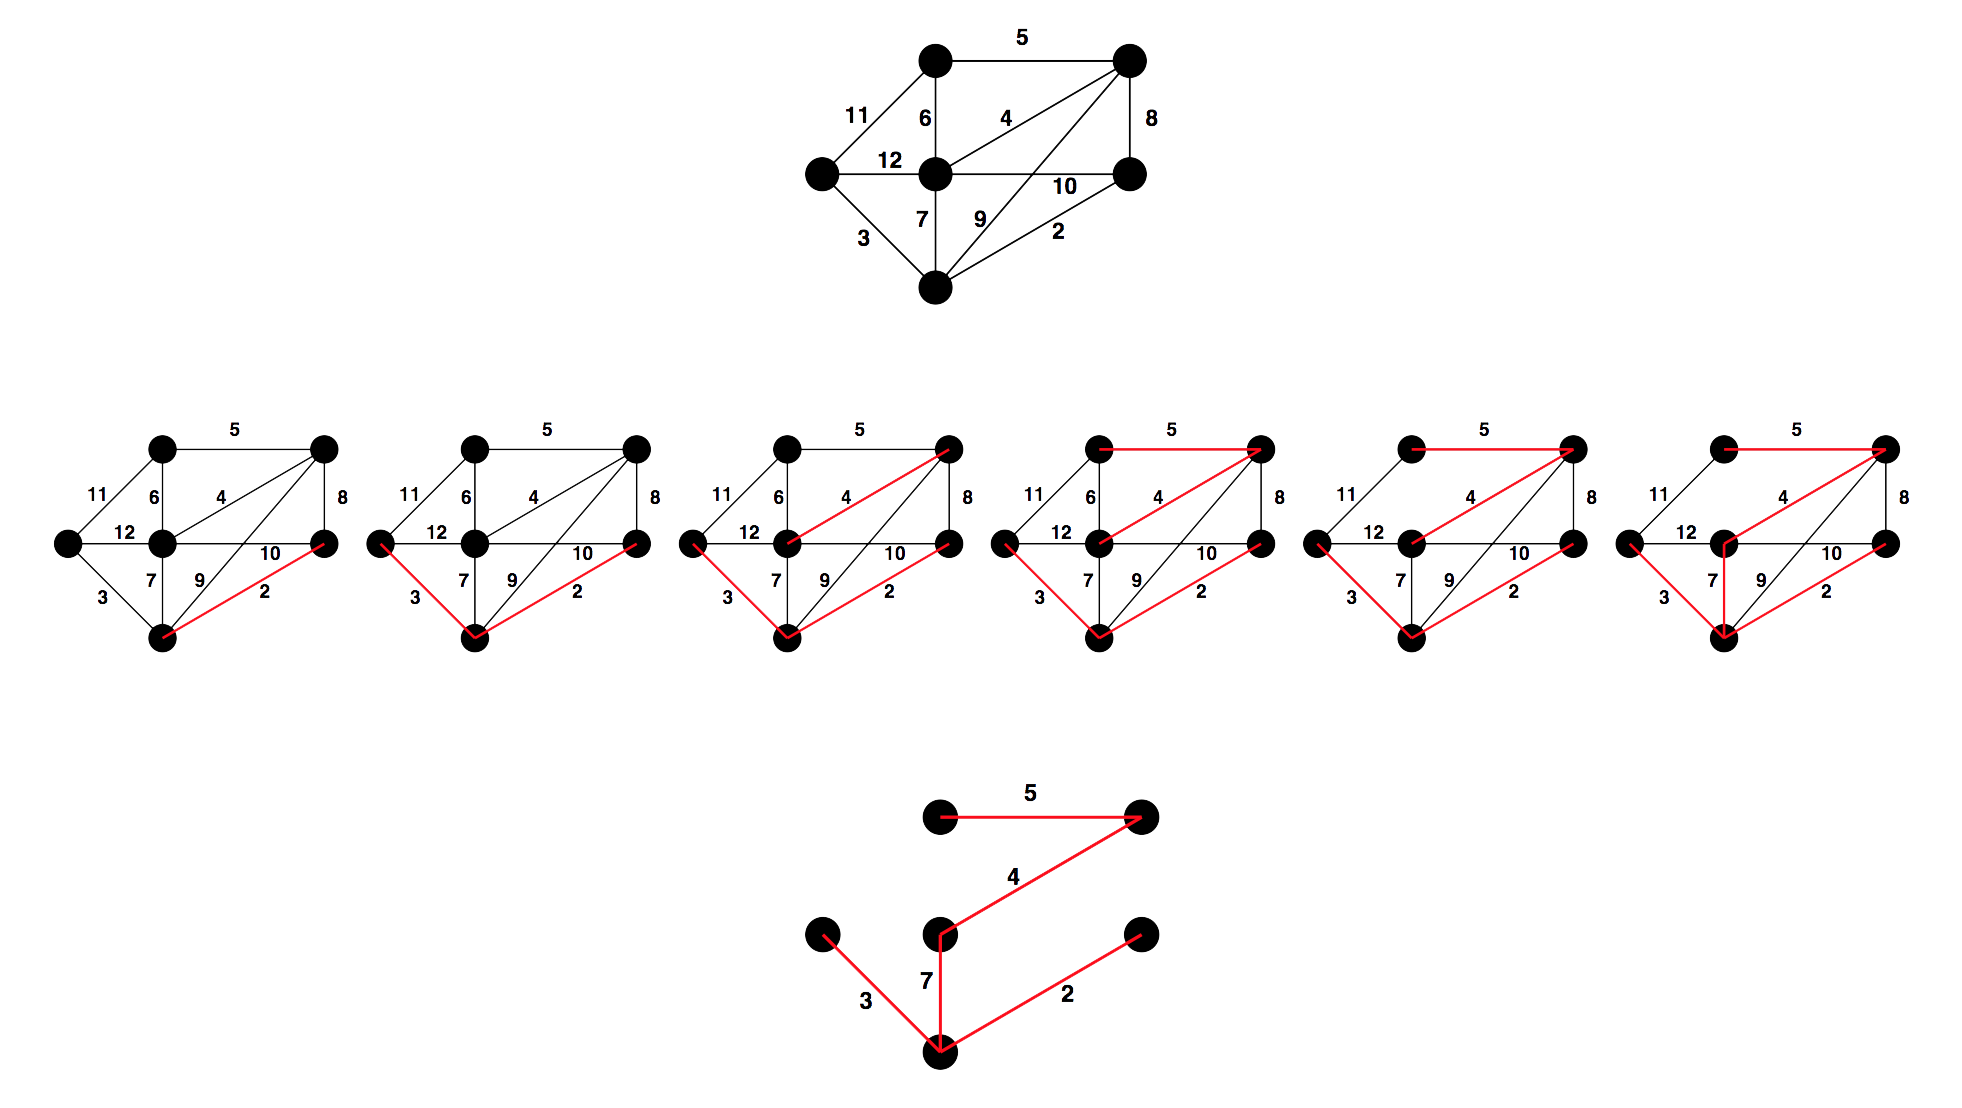
\includegraphics[width=400pt]{../img/kruskal}
  \end{center}
\end{myexem}

\begin{mytheo}
  L'algorithme de Kruskal est correct.
  \begin{proof}
    Soit $T$ l'arbre trouvé par Kruskal,
    c'est bien un arbre sous-tendant car il a $n-1$ arêtes et qu'il n'a pas de cycle.
    Démontrons qu'il est optimal par l'absurde.

    S'il ne l'est pas, c'est qu'il existe un arbre sous-tendant $T^*$ tel que $w(T^*) < w(T)$.
    Soit $e$ la plus petite arête telle que $T$ l'a et $T^*$ ne l'a pas ou le contraire.
    \begin{itemize}
      \item Si $T$ ne l'a pas et que $T^*$ l'a, ça veut dire qu'elle crée un cycle avec les
        arête de poids strictement plus petit qui sont dans $T$.
        Ces arêtes sont aussi dans $T^*$ car on a considéré que c'était la plus petite qui différait.
        Pourtant $T^*$ n'a pas de cycle car c'est un arbre. On est donc pas dans ce cas là.
      \item On sait donc que $T$ l'a et que $T^*$ ne l'a pas.
        Comme $T^*$ est un arbre, $T^* + e$ a un et un seul cycle.
        Dans ce cycle, il y a nécessairement des arête que $T$ n'a pas car $T$ a $e$ et qu'il n'a pas de cycle.
        Ces arêtes on un poids plus grand ou égal à $e$ car on a dit qu'on prenait $e$ avec le poids
        le plus petit qui différait entre $T$ et $T^*$. Soit $e'$, l'une d'entre elle.
        Comme $T^*+e$ a un et un seul cycle et que $e'$ est dedans, $T^*+e-e'$ est un arbre sous-tendant.

        Si $w(e) < w(e')$, on arrive à une contradiction.
        Si $w(e) = w(e')$, on prends ${T^*}'=T^*+e-e'$ qui est aussi
        un graphe sous-tendant de poids minimum car $w({T^*}') = w(T^*+e-e') = w(T^*)+w(e)-w(e') = w(T^*)$.
        Si ${T^*}' = T$, on a notre contradiction, sinon on recommence le raisonnement.
        On ne pourra pas le recommencer indéfiniment car il y a un nombre fini d'arête qui diffère entre $T^*$
        et $T$ et à chaque fois, il y en a une de moins qui diffère.
    \end{itemize}
    $T$ est donc optimal.
   \end{proof}
\end{mytheo}

\begin{mytheo} [L'algorithme de Kruskal est efficace]
  L'algorithme de Kruskal requiert un temps de calcul de l'ordre de $\bigoh(m\log(m))$ sur un graphe à $m$ arêtes.
  \begin{proof}
    On doit commencer par trier les arêtes du graphes ce qui se fait en $\bigoh(m\log(m))$ avec un algorithme efficace.
    Savoir si ajouter une arête crée un cycle se fait en $\bigoh(\alpha(m))$ avec un Union-Find.
    On retient pour chaque noeud dans quel composante connexe il est.
    Une arête crée un cycle si et seulement si ses deux extrémités sont dans la même composante connexe,
    ce qui se fait à l'aide de deux \emph{find} en $\bigoh(\alpha(m))$.
    Lorsqu'on ajoute une arête, on fait l'union de deux composantes connexes,
    ce qui se fait en $\bigoh(\alpha(m))$ à l'aide d'une \emph{union}.
    \footnote{$\alpha(m)$ est la réciproque de la fonction $f(n) = A(n,n)$ et
    $A$ la fonction d'Ackermann dont la croissance est extrêmement rapide.
    $\alpha(m)$ vaut moins de 5 pour toute valeur $m$ en pratique.}
  \end{proof}
\end{mytheo}

\index{coupe de sommets}
\begin{mydef}
  Pour un graphe connexe, une \emph{coupe de sommets} est un ensemble de sommets qui déconnecte le graphe quand on l'en retire.
\end{mydef}

\index{coupe d'arêtes}
\begin{mydef}
  Pour un graphe connexe, une \emph{coupe d'arêtes} est un ensemble d'arêtes qui déconnecte le graphe quand on l'en retire.
\end{mydef}

\index{graphe!graphe k-connexe}
\begin{mydef}
  Un graphe est dit \emph{k-connexe} si retirer $k − 1$ noeuds quelconques laisse le graphe connexe. Autrement dit, si toutes les coupes de sommets sont de taille au moins $k$.
\end{mydef}

\index{connectivité}
\begin{mydef}
   La \emph{connectivité} d'un graphe est la taille de la plus petite coupe de sommets. Si tous les $n$ noeuds sont voisins (ex., le graphe complet), la connectivité est définie comme $n − 1$.
\end{mydef}

\index{graphe!graphe k-arête-connexe}
\begin{mydef}
   Un graphe est dit \emph{k-arête-connexe} si retirer $k − 1$ arêtes quelconques laisse le graphe connexe. Autrement dit, si toutes les coupes d'arêtes sont de taille au moins $k$.
\end{mydef}

\index{connectivité!arête-connectivité}
\begin{mydef}
   L'\emph{arête-connectivité} d'un graphe est la taille de la plus petite coupe d'arêtes.
\end{mydef}

\begin{mytheo} [Lien entre les connectivités]
  $$ \text{connectivité} \leq \text{arête-connectivité} \leq \text{degré minimum}$$
  \begin{proof}
    \noindent
    $$\text{arête-connectivité} \leq \text{degré minimum}$$
    Est une façon de déconnecter un graphe est de retirer les arêtes incidentes au noeud de degré minimum
    
    $$\text{connectivité} \leq \text{arête-connectivité}$$
    Par récurrence (le cas arête-connectivité = 0 est trivial). On prend une coupe de k arêtes (avec e qui est une arête quelconque de cette coupe). G-e a, par conséquent, une arête-connexité k-1. 
    \begin{itemize}
      \item Cas extrême : G-e a tous les noeuds adjacents (graphe complet avec, éventuellement, répétition d'arêtes). Alors : $\text{connectivité(G)}=\text{connectivité(G-e)} \leq k-1$.
      \item Sinon, il existe une coupe de sommets S de G-e telle que G-e-S est déconnecté.
        Si G-S est déjà déconnecté, alors $\text{connectivité(G)} \leq |S| \leq k - 1 \leq k$.

        Si G-S est connecté, alors e est une coupe d'arête puisque G-S-e est déconnecté.

        Si il y a au moins 3 noeuds x,u,v dans G-S: alors en retirant u ou v, on déconnecte x de v ou de u.
        Donc,
        $S \cup \{u \text{ou} v\}$ est une coupe de G et $\text{connectivité}(G) \leq |S| + 1  \leq k$
    \end{itemize}
 \end{proof}
\end{mytheo}

\begin{mytheo} [Théorème de Whitney]
  Un graphe à au moins trois noeuds est 2-connexe ssi toute paire de noeuds distincts est reliée par au moins deux chemins dont les noeuds internes sont distincts.
  \begin{proof}
   \fbox{$\Longleftarrow$}
   \newline
   Si je retire un noeud quelconque du graphe, $\forall u,v$ au plus 1 des 2 chemin est toujours connecté $\rightarrow$ G reste connexe. \\
   \fbox{$\Longrightarrow$}
     \newline
     Par récurrence sur $d(u,v)$ : 
     \begin{enumerate}
     \item Cas de base : $d(u,v)=1$. Si G est 2-connexe alors G est 2-arête-connexe (cfr théorème précédent) donc retirer une arête laisse le graphe connexe. Soit l'arête e telle qu'il existe le chemin uev. Si on retire e, u et v sont toujours connecté donc existe donc un chemin P tel que uPv. $\rightarrow$ 2 chemins entre u et v.
     \item Si c'est vrai pour toute paire de noeuds $x,y$ tels que $d(x,y) < d(u,v)$, prouvons que c'est également vrai pour $d(u,v)$. Soit $w$, le dernier noeud sur le chemin le plus court de u à v. Par hypothèse, $d(u,w) < d(u,v)$ et par récurrence, u et w sont reliés par au moins 2 chemins dont les noeuds internes sont distincts, nommons les $P_1$ et $P_2$. Si je retire w, il existe, par connexité, un chemin P de u à v qui ne passe pas par w. Soit x le dernier noeud de P qui appartient à $P_1$ ou à $P_2$ (éventuellement, x=u). Il existe donc 2 chemins de u à v : u \dots x\dots v, et u \dots w \dots v. Par construction, ces chemins sont disjoints. 
     \end{enumerate}
  \end{proof}
\end{mytheo}

Ce théorème se généralise :

\begin{mytheo} [Théorème de Menger]
  Un graphe à au moins $k + 1$ noeuds est k-connexe ssi toute paire de noeuds distincts est reliée par au moins deux chemins dont les noeuds internes sont distincts.
  \begin{proof}
     Preuve \addTODO
  \end{proof}
\end{mytheo}

\begin{mytheo} [Nombre d'arêtes dans un graphe k-connexe]
  Tout graphe k-connexe à $n$ noeuds possède $kn/2$ arêtes au moins (condition nécessaire).
  \begin{proof}
     k-connexe $\rightarrow$ degré min $\geq$ k $\rightarrow$ $\sum \text{degrés} \geq kn \ \rightarrow \ |E| \geq kn/2$.
  \end{proof}
\end{mytheo}

\begin{mytheo} [Théorème de Harary]
  Le graphe de Harary $H_{k ,n}$ possède $kn/2$ arêtes et est k-connexe.
  \begin{proof}
     Preuve \addTODO
  \end{proof}
\end{mytheo}

\begin{myexem}
  Exemples de graphes de Harary ($H_{4,8}$ ici) :
	\begin{center}
    	  \begin{tikzpicture}[scale = 1]
          \node[draw, circle] at ( 0, 4)  (0) {0};
					\node[draw, circle] at ( 3,3) (1) {1};
          \node[draw, circle] at ( 4, 0  )  (2) {2};
          \node[draw, circle] at ( 3,-3)  (3) {3};
          \node[draw, circle] at (0,-4)  (4) {4};
          \node[draw, circle] at (-3, -3)  (5) {5};
					\node[draw, circle] at (-4, 0  )  (6) {6};
					\node[draw, circle] at (-3, 3)  (7) {7};

					\draw[-] (0) edge node {} (1);
					\draw[-] (0) edge node {} (2);
					\draw[-] (0) edge node {} (6);
					\draw[-] (0) edge node {} (7);
					\draw[-] (1) edge node {} (7);
          \draw[-] (1) edge node {} (2);
					\draw[-] (1) edge node {} (3);
          \draw[-] (2) edge node {} (3);
					\draw[-] (2) edge node {} (4);
          \draw[-] (3) edge node {} (4);
					\draw[-] (3) edge node {} (5);
          \draw[-] (4) edge node {} (5);
					\draw[-] (4) edge node {} (6);
          \draw[-] (5) edge node {} (6);
					\draw[-] (5) edge node {} (7);
					\draw[-] (6) edge node {} (7);
        \end{tikzpicture}
 \end{center}
\end{myexem}

\section{Graphes hamiltoniens}
\subsection{Graphes hamiltoniens}
\index{chemin!chemin hamiltonien}
\begin{mydef}
  Un \emph{chemin} est \emph{hamiltonien} s’il passe par chaque noeud du graphe une et une seule fois.
\end{mydef}

\index{cycle!cycle hamiltonien}
\begin{mydef}
  Un \emph{cycle} est \emph{hamiltonien} s’il passe par chaque noeud du graphe une et une seule fois.
\end{mydef}

\index{graphe!graphe hamiltonien}
\begin{mydef}
  Un \emph{graphe} est \emph{hamiltonien} s’il possède un cycle hamiltonien.
\end{mydef}

\begin{mytheo} [Condition nécessaire pour un graphe hamiltonien]
  Si on ôte $k$ noeuds quelconques d’un graphe hamiltonien, on obtient au plus $k$ composantes connexes.
  \begin{proof}
     Soit $v_1 ... v_nv_1$, le cycle hamiltonien.\\
     Retirer $k$ noeuds du cycle laisse $\leq k$ composantes (=morceaux du cycle connexes), on crée au plus $k$ chemins, tous les noeuds sur un même chemin sont dans une même composante connexe. Les autres arêtes ne peuvent que diminuer encore le nombre de composantes connexes.
  \end{proof}
\end{mytheo}
\begin{myexem} Le graphe suivant est bien hamiltonien.
  \begin{figure} [!h]
      \hspace*{\fill}
         \subfigure[]
         {
             \begin{tikzpicture}[scale = 0.5]
          	 \fill[black] (-1,0) circle (0.1cm);
          	 \fill[black] (-2,2) circle (0.1cm);
          	 \fill[black] (-1.5,4) circle (0.1cm);
          	 \fill[black] (-2.5,5) circle (0.1cm);
          	 \fill[black] (0,6) circle (0.1cm);
          	 \fill[black] (2.5,4.5) circle (0.1cm);
          	 \fill[black] (2.5,2) circle (0.1cm);
          	 \fill[black] (3,1) circle (0.1cm);
          	 \fill[black] (1.5,0) circle (0.1cm);

          	 \draw (-1,0) -- (-2,2) -- (-1.5,4) -- (-2.5,5) -- (0,6) -- (2.5,4.5) -- (2.5,2) -- (3,1) -- (1.5,0) -- cycle;
        \end{tikzpicture}
      	}
      	\hfill
      \subfigure[] 
         {
             \begin{tikzpicture}[scale = 0.5]
          	 \fill[black] (-1,0) circle (0.1cm);
          	 \fill[black] (-2,2) circle (0.1cm);
          	 \fill[black] (-2.5,5) circle (0.1cm);
          	 \fill[black] (0,6) circle (0.1cm);
          	 \fill[black] (2.5,2) circle (0.1cm);
          	 \fill[black] (3,1) circle (0.1cm);

             \draw (-2.5,5) -- (0,6);
          	 \draw (-1,0) -- (-2,2);
          	 \draw (2.5,2) -- (3,1);
        \end{tikzpicture}
      	}
      	\hspace*{\fill}
    \end{figure} \newline
    En retirant 3 noeuds du graphe $g$ on obtient bien 3 composantes connexes dans le graphe $h$.
\end{myexem}

\begin{mytheo} [Condition suffisante pour un graphe hamiltonien]
  Un graphe simple à $n \geq 3$ noeuds tel que le degré minimum est d’au moins $n/2$ est hamiltonien.
  \begin{proof}
     Par l'absurde.

     Supposons qu'il existe un graphe à $n \geq 3$ noeuds de degré minimum $d(v) \geq \frac{n}{2}$ non hamiltonien.

     Prenons un tel graphe qui est maximal pour cette propriété : ajouter une arête dans ce graphe le rendrait hamiltonien.

     Ce graphe G n'est pas le graphe complet $K_n$
     \begin{align*}
		&\Rightarrow \exists \text{ des noeuds } v_1, v_n \text{ non adjacents} \\
		&\Rightarrow G + \{v_1, v_n \} \text{ est hamiltonien} \\
		&\Rightarrow \exists \text{ un cycle hamiltonien passant par l'arête } v_1v_n \\
		&\Rightarrow \text{Dans } G, \exists \text{ un chemin hamiltonien } v_1v_2...v_n
	\end{align*}
	Considérons les ensembles:
	\begin{align*}
		S &= \{v_i \mid v_{i+1} \text{ est adjacent à } v_1\} &\vert S \vert = \text{degré}(v_1) \geq \frac{n}{2}\\
		T &= \{v_i \mid v_{i} \text{ est adjacent à } v_n\} &\vert T \vert = \text{degré}(v_n) \geq \frac{n}{2}
	\end{align*}
	On sait que $v_n \not\in S$, par hypothèse $v_1$ et $v_n$ ne sont pas adjacents, et $v_n \not\in T$. On a donc $\vert S \cup T \vert < n$ puisqu'aucun des ensembles ne contient $v_n$.
	De plus, $\vert S \cap T \vert = \emptyset $ : en effet, si $\exists v_i \in \vert S \cap T \vert$, alors $v_1v_2...v_iv_nv_{n-1}...v_{i+1}v_1$ est un cycle hamiltonien $\Rightarrow$ Contradiction
	\begin{figure} [!h]
		\center
        \begin{tikzpicture}[scale = 0.5]
          	 \fill[black] (-7,0) circle (0.3cm);
          	 \node at (-7,-1) {$v_1$};
          	 \fill[black] (-5,0) circle (0.3cm);
          	 \node at (-5,-1) {$v_2$};
          	 \fill[black] (-1,0) circle (0.3cm);
          	 \node at (-1,-1) {$v_i$};
          	 \fill[black] (1,0) circle (0.3cm);
          	 \node at (1,1) {$v_{i+1}$};
          	 \fill[black] (5,0) circle (0.3cm);
          	 \node at (5,1) {$v_{n-1}$};
          	 \fill[black] (7,0) circle (0.3cm);
          	 \node at (7,1) {$v_n$};

          	 \draw (-7,0) -- (-5,0);
          	 \draw [dashed] (-5,0) -- (-1,0);
          	 \draw [dashed] (1,0) -- (5,0);
          	 \draw (5,0) -- (7,0);
          	 \draw (1,0) to[bend right] (-7,0);
          	 \draw (-1,0) to[bend right] (7,0);
        \end{tikzpicture}
    \end{figure}
	\newline \newline
	Enfin, $\vert S \cup T \vert = \vert S \vert + \vert T \vert - \vert S \cap T \vert \geq n$ mais $\vert S \cup T \vert < n$ $\Rightarrow$ Contradiction
  \end{proof}
\end{mytheo}

\index{problème}
\index{problème!du postier chinois}
\begin{mydef} [Problème du postier chinois]
  Dans un graphe pondéré, trouver le parcours fermé le plus court qui passe par toutes les arêtes au moins une fois.
\end{mydef}

\index{problème!du voyageur de commerce}
\begin{mydef} [Problème du voyageur de commerce]
  Dans un graphe pondéré, trouver le parcours fermé le plus court qui passe par tous les noeuds au moins une fois.
\end{mydef}

\section{Séance 5}

\textbf{Graphes Hamiltoniens}

\subsection{Cycle hamiltonien et eulerien}
Pour quelle classe de graphes un tour eulérien est-il aussi hamiltonien? Peut-on en déduire une caractérisation des graphes qui sont à la fois eulériens et hamiltoniens?
\begin{solution}
\begin{itemize}
\item Pour les graphes connexes dont tous les noeuds sont de degré 2.
\item Pour avoir un graphe qui est à la fois eulérien et hamiltonien, il faut partir du cycle hamiltonien de base. Si on décide d'ajouter des arêtes, il faut respecter la condition ``garder le degré pair''. En effet, le cycle hamiltonien n'est pas spécialement le même que le cycle eulérien.
\end{itemize}
\end{solution}

\subsection{Problème du cavalier}
Le problème du cavalier était un problème en vogue au XVIIIème siècle. Le problème est de déterminer s'il est possible de faire parcourir toutes les cases d'un échiquier de taille $n \times n$ à un cavalier en ne passant qu'une seule fois par chaque case et en revenant à son point de départ. Formulez cela comme un tour hamiltonien dans un graphe et montrez que la réponse est négative pour $n$ impair.
\begin{solution}
Ce problème correspond à trouver un tour hamiltonien dans un graphe dans lequel les sommets sont les cases du graphe. Les sommets sont reliés entre eux lorsque le cavalier peut se déplacer d'un à l'autre directement.\\
Comme le mouvement du cavalier lui permet de se déplacer uniquement d'une case blanche à une case noire et d'une case noire à une case blanche, ce graphe est biparti.
Si $n$ est impair, le nombre de cases est impair également et le problème demande donc de trouver un cycle hamiltonien de longueur impaire dans un graphe biparti. Hors, un graphe est biparti si et seulement si il ne contient aucun cycle de longueur impaire. Il est donc impossible de résoudre ce problème si n est impair.
\textit{\textsc{En bref: }Dans un graphe biparti, si le nombre de noeuds n'est pas le même des deux côtés, le graphe n'est pas hamiltonien.}
\end{solution}

\subsection{Théorème de Dirac}
Le théorème de Dirac affirme que si $d(v) > n/2$ pour tous les sommets $v \in V$ d'un graphe $G=(V,E)$, alors $G$ est hamiltonien. Donnez un graphe hamiltonien de $n$ sommets qui ne satisfait pas les conditions du théorème de Dirac. Donnez un graphe qui n'est pas hamiltonien et qui satisfait $d(v) \geq (n-1)/2$ pour tout $v \in V$.

\begin{solution}
\begin{itemize}
\item Graphe hamiltonien de 5 sommets ne satisfaisant pas les conditions du théorème de Dirac.\\
\includegraphics[scale=0.5]{ape5_ex3_1.png}
\item Graphe non hamiltonien de 5 sommets satisfaisant $d(v) \geq (n-1)/2$ pour tout $v \in V$.\\
\includegraphics[scale=0.5]{ape5_ex3_2.png}
\end{itemize}
\end{solution}

\subsection{Double cycle hamiltonien}
Placez $n$ sommets sur un cercle et liez un sommet à ses deux plus proches voisins dans les deux directions. Démontrez que pour $n \geq 5$ le graphe obtenu est l'union de deux circuits hamiltoniens.

\begin{solution}
Pour $n$ impair, ce résultat est évident. On a le circuit hamiltonien intérieur (en vert) et celui extérieur (en rouge).\\
\includegraphics[scale=0.5]{nimpair.jpg}
\\
Pour $n$ pair, on propose une méthode de construction des 2 circuits hamiltoniens qui fonctionne pour tout $n$ pair. On commence par construire, pour $n=6$ le graphe suivant, avec le circuit hamiltonien intéreur (en vert) et celui extérieur (en rouge).
\\
\includegraphics[scale=0.5]{npair1.jpg}
\\
Il est très facile d'ajouter les noeuds par 2 en complétant les circuits hamiltoniens. On construit d'abord le circuit extérieur (en rouge) en gardant toujours la même façon de procéder, et ensuite celui intérieur, qui comprend les arêtes non-utilisées par le circuit rouge. Voici le graphe pour $n=8$.
\\
\includegraphics[scale=0.5]{npair2.jpg}
\\
\end{solution}

\subsection{Souris VS gruyère}
\paragraph{solution 1 :}
Une souris mange un gruyère de dimension $3 \times 3 \times 3$ par petits morceaux de taille $1 \times 1 \times 1$. Elle démarre en un coin du cube et se déplace de cube adjacent en cube adjacent. Peut-elle manger la totalité du gruyère en terminant par le cube central?
\begin{solution}
La justification est la même que pour le problème du cavalier. Modélisons le fromage comme un graphe dont chaque cube de dimension $1 \times 1 \times 1$ est un noeud et dont les noeuds représentant des cubes adjacents sont reliés par une arête.\\
En effet, ce graphe est biparti. On peut imaginer peindre le noeud de départ en blanc, ceux qui y sont adjacents en noir, ceux adjacents à ceux-ci en blanc etc.\\
Le nombre de noeuds peints en blanc sera donc 14 et ceux peints en noir 13. Il est évidemment impossible de trouver un chemin hamiltonien partant d'un coin (blanc) et se terminant au centre (noir) et ayant parcouru tous les noeuds.
En d'autre termes, il n'est alors possible de construire un cycle qui passe par tous les noeuds et qui revient au point de départ. 
\paragraph{solution 2 :}
Une autre manière de voir les choses est d'utiliser la condition nécessaire sur les graphe hamiltoniens: si on supprime les 13 noeuds, on obtient 14 composantes connexes. Or si un graphe est hamiltonien, supprimer $k$ noeuds crée au plus $k$ composantes connexes. On a une contradiction et donc le graphe n'est pas hamiltonien.
\end{solution}

\subsection{Borne d'un voyageur de commerce}
Trouvez des bornes supérieures et inférieures sur la valeur optimale du problème du voyageur de commerce avec les distances suivantes (les distances satisfont l'inégalité triangulaire) :
\begin{equation}
  \left( \begin{matrix}
      - & 5 & 4 & 3 & 6 \\
      - & - & 6 & 4 & 5 \\
      - & - & - & 3 & 3 \\
      - & - & - & - & 5 \\
      - & - & - & - & -
  \end{matrix}  \right)
\end{equation}
\begin{solution}
Une borne supérieure de la solution optimale est obtenue en faisant par exemple le parcours 1-2-3-4-5: $5+4+3+6=18$\\
Une borne inférieure peut être obtenue en additionnant les 4 plus petites distances entre les villes: $3+3+4+4=12$\\
\end{solution}

\subsection{Ordonancement de taches sur une machine spécialisée}
Formulez le problème suivant comme le problème du voyageur de commerce. Cinq opérations $j=1,…,5$ doivent avoir lieu sur une machine spécialisée. Les temps de transition $c_{ij}$ entre deux opérations sont importants, et sont donnés dans la table suivante:
\begin{equation}
  \left( \begin{matrix}
      10 & 23 & 42 & 11 & 24 \\
      19 & 13 & 42 & 36 & 43 \\
      67 & 34 & 23 & 29 & 21 \\
      19 & 52 & 41 & 37 & 31 \\
      96 & 63 & 75 & 89 & 43
  \end{matrix}  \right)
\end{equation}
En plus, si une opération $j$ est en première position, il faut aussi un temps de préparation $t_j$ qui est fonction de l'opération, où $t=(23,41,32,54,11)$. Pour des raisons techniques, on décide que l'opération $3$ ne peut pas précéder directement l'opération $1$, et les opérations $4$ et $5$ ne peuvent pas avoir lieu en dernière position.

\begin{solution}
Ce problème peut être modélisé comme le problème du voyageur de commerce dans un graphe orienté.
\begin{itemize}
\item Les opérations (par lesquelles il faut toutes passer) représentent les villes et sont modélisées comme des noeuds. 
\item Les arêtes sont les temps de transitions entre les opérations et relient ces opérations en étant dirigées de l'opération de départ  celle d'arrivée. Leur poids est le temps de transition. Elles représentent les routes dans le problème du voyageur de commerce.
\item On ajoute un noeud de départ, qui est relié à toutes les opérations par des arêtes qui ont des poids valant les temps de préparations respectifs des opérations et en étant dirigées vers les opérations. 
\item On ajoute également un noeud d'arrivée, auquel sont reliées toutes les opérations à l'aide d'arêtes de poids nuls en étant dirigée vers ce noeud.
\item Afin de modéliser la condition ``L'opération 3 ne peut pas précéder directement l'opération 1'', on supprime l'arête partant de l'opération 3 et allant vers l'opération 1.
\item Afin de modéliser la condition ``les opérations 4 et 5 ne peuvent pas avoir lieu en dernière position'', on supprime les arêtes qui partent des opérations 4 et 5 sont dirigées vers le noeud d'arrivée
\end{itemize}
\end{solution}

\subsection{Diner en territoire ennemi}
Un groupe de huit personnes se retrouve pour diner. Le graphe ci-dessous précise les ``incompatibilités d'humeur'' entre les personnes de ce groupe (une arête reliant deux personnes indique que celles-ci s'entendent très modérément). Proposez un plan de table (la table est ronde) pour ce groupe en évitant de placer côte à côte deux personnes ``incompatibles''.

\begin{figure}[h!]
  \begin{center}
    \begin{tikzpicture}[-,>=stealth',shorten >=1pt,auto]
      \Vertex[x=0 ,y=0]{8}
      \Vertex[x=0 ,y=-2]{7}
      \Vertex[x=2,y=1]{1}
      \Vertex[x=2 ,y=-3]{6}
      \Vertex[x=4 ,y=1]{2}
      \Vertex[x=4 ,y=-3]{5}
      \Vertex[x=6 ,y=0]{3}
      \Vertex[x=6 ,y=-2]{4}


      \path[every node/.style={font=\sffamily\small}]
      (1) edge node [left] {} (2)
      edge node [left] {} (4)

      (2) edge node [right] {} (5)
      edge node [right] {} (6)
      edge node [right] {} (8)

      (3) edge node [right] {} (4)
      edge node [left] {} (5)

      (4) edge node [right] {} (7)

      (5) edge node [right] {} (6)

      (6) edge node [right] {} (8)

      (7) edge node [left] {} (8);

    \end{tikzpicture}
  \end{center}
\end{figure}

\begin{solution}
Afin de trouver un plan de table qui conviendrait, il faut d'abord créer le complémentaire du graphe précédent. Dans celui-ci, les arêtes relient deux personnes qui s'entendent bien. Il faut ensuite trouver un cycle hamiltonien dans ce graphe, et l'ordre dans lequel les noeuds sont parcourus sera celui dans lequel les gens sont placés autour de la table. Une solution possible est la suivante:$1-3-6-4-2-7-5-8$
\end{solution}

\section{Coloriages d'arêtes}
\subsection{Coloriages d'arêtes}
%il manque encore qq définitions

%dessin d'un graphe avec professeur et classes
\paragraph{Problème des horaires}
Chaque professeur doit enseigner à un certain nombre de classes pendant un certain nombre d'heures. On veut créer
un horaire sur le plus petit nombre de période possible
\\On relie chaque professeur aux classes auxquelles il donne cours en veillant a colorier les arêtes en fonction des tranches horaires. Deux arêtes de la même couleur ne peuvent pas partir du même nœud.

\index{coloriage}
\index{coloriage!coloriage d'arêtes}
\index{coloriage!coloriage d'arêtes propre}
\begin{mydef}
  Un \emph{coloriage} des arêtes d’un graphe en k couleurs est l’assignation à chaque arête d’une couleur 1; 2; ..., ou $k$. Ce coloriage est dit \emph{propre} si deux arêtes adjacentes sont toujours de couleurs différentes.
\end{mydef}

\index{chromatique!indice chromatique}
\begin{mydef}
  L’\emph{indice chromatique} d’un graphe $G$, noté $\chi '$ ($G$) est le nombre minimal de couleurs nécessaire pour obtenir un coloriage propre des arêtes de $G$.
\end{mydef}


\begin{mytheo}[König]
  Pour tout graphe biparti: $\chi '= degré\ max$
  \begin{proof}
    On va utiliser le théorème de Hall pour les graphes bipartis réguliers (qui ont toujours un couplage parfait).
    \begin{enumerate}


    \item Soit un graphe biparti $k$-régulier. Par le théorème de Hall, il existe un couplage parfait. On le colorie en couleur $c_{1}$. On considère ensuite les arêtes restantes non encore coloriées: elles forment un graphe $k-1$ régulier. On recommence pour la couleur $c_{2}$ avec un autre couplage. On continue jusqu'à épuisement, on obtient alors $\chi '=k$
    \item Pour un graphe biparti quelconque de degré $k$.
    \begin{itemize}
    \item Ajouter des nœuds d'un côté si nécessaire pour avoir le même nombre de nœuds de chaque côté.
    \item Si tous les nœuds ne sont pas de degré $k$, alors il y a au moins 1 nœuds de degré $<k$ de chaque côté. On ajoute alors une arête entre eux. On recommence jusqu'à $k$-régularité.
    \end{itemize}
    Par le point 1. , il existe un coloriage propre à $k$ couleurs. On supprime ensuite les arêtes et nœuds ajoutés: on obtient un coloriage propre pour le graphe de départ.
    $$\Rightarrow deg max \le \chi ' \le k=deg max$$
    $$\Rightarrow \chi ' = k$$
    \end{enumerate}
  \end{proof}
\end{mytheo}

\begin{mytheo} [Vizing]
Pour tout graphe simple: $\chi ' = deg max$ ou  $\chi ' = deg max + 1$
  \begin{proof} On sait que $\chi' \ge deg max$, il faut donc prouver que $\chi ' \le deg max + 1$.
  \\On le prouve par induction sur le nombre d'arêtes du graphe.
  \\ \textbf{Pas inductif:} Vrai pour $m$ arêtes. Soit un graphe à  $m+1$ arêtes, de degré max $k$. Je retire une de ces arêtes: il existe un coloriage propre à $\le k+1$ couleurs.
  \begin{itemize}
  \item Si $\le k$ couleurs: je choisis (k+1) couleurs pour la $(m+1)^{ième}$ arête.
  \item Si $k+1$ couleurs $c_{1},...,c_{k+1}$: je rétablis la $(m+1)^{ième}$ arête: il faut trouver une couleur pour cette arête.
  \end{itemize}

  \end{proof}
\end{mytheo}
\textbf{Observation:} En chaque nœud il y a au moins une couleur libre (c'est à dire pas utilisée par les arêtes incidentes)
\\
\newline Voici 3 exemples avec $k=3$ et 4 couleurs \emph{noir, bleu, rouge et vert}
\begin{myexem} \label{exemple1}
  Même couleur libre \emph{rouge} pour $x$ et $y$ $\Rightarrow$ on peut utiliser le \emph{rouge} pour $xy$
  \begin{figure}[H]
    \begin{center}
      \subfigure[]{
        \begin{tikzpicture}[scale = 1]
          \draw[thick,black] (0,1) -- (2,1.5);
          \draw[thick,blue] (0,1) -- (2,0.5);
          \draw[thick,dotted,black] (0,1) -- (0,-1);
          \draw[thick,black] (0,-1) -- (2,-0.5);
          \draw[thick,blue] (0,-1) -- (2,-1.5);

          \node at (-0.25,1) {$x$};
          \node at (-0.25,-1){$y$};
        \end{tikzpicture}
      }
      \subfigure[]{
        \begin{tikzpicture}[scale = 1]
          \draw[thick,black] (0,1) -- (2,1.5);
          \draw[thick,blue] (0,1) -- (2,0.5);
          \draw[very thick,red] (0,1) -- (0,-1);
          \draw[thick,black] (0,-1) -- (2,-0.5);
          \draw[thick,blue] (0,-1) -- (2,-1.5);

          \node at (-0.25,1) {$x$};
          \node at (-0.25,-1){$y$};
        \end{tikzpicture}
      }
    \end{center}
  \end{figure}
\end{myexem}

\begin{myexem}
  Pas de couleur libre entre $x$ et $y$. Mais le \emph{noir} est libre pour $y$\\
  $\Rightarrow$ on utilise le \emph{noir} pour $xy$, on efface l'arête \emph{noir} $xy'$\\
  $\Rightarrow$ On se retrouve dans le cas \ref{exemple1}, on utilise ensuite la couleur \emph{vert} pour $xy'$\\
  \begin{figure}[H]
    \begin{center}
      \subfigure[]{
        \begin{tikzpicture}[scale = 1]
          \draw[thick,red] (0,1) -- (2,1.5);
          \draw[thick,green] (0,1) -- (2,0.5);
          \draw[thick,dotted,black] (0,1) -- (0,-1);
          \draw[thick,black] (0,-1) -- (2,-0.5);
          \draw[thick,blue] (0,-1) -- (2,-1.5);
          \draw[thick,blue] (2,-0.5) -- (4,0);
          \draw[thick,red] (2,-0.5) -- (4,-1);

          \node at (-0.25,1) {$y$};
          \node at (-0.25,-1){$x$};
          \node at (1.90,-0.25){$y'$};
        \end{tikzpicture}
      }
      \subfigure[]{
        \begin{tikzpicture}[scale = 1]
          \draw[thick,red] (0,1) -- (2,1.5);
          \draw[thick,green] (0,1) -- (2,0.5);
          \draw[very thick,black] (0,1) -- (0,-1);
          \draw[thick,dotted,black] (0,-1) -- (2,-0.5);
          \draw[thick,blue] (0,-1) -- (2,-1.5);
          \draw[thick,blue] (2,-0.5) -- (4,0);
          \draw[thick,red] (2,-0.5) -- (4,-1);

          \node at (-0.25,1) {$y$};
          \node at (-0.25,-1){$x$};
          \node at (1.90,-0.25){$y'$};
        \end{tikzpicture}
      }
    \end{center}
  \end{figure}
\end{myexem}

\begin{myexem}
  Quelques fois cette astuce ne suffit pas:\\
  \begin{figure}[H]
    \begin{center}
	    \begin{tikzpicture}[scale = 1]
        \draw[thick,red] (0,1) -- (2,1.5);
        \draw[thick,green] (0,1) -- (2,0.5);
        \draw[thick,dotted,black] (0,1) -- (0,-1);
        \draw[thick,black] (0,-1) -- (2,-0.5);
        \draw[thick,blue] (0,-1) -- (2,-1.5);
        \draw[thick,green] (2,-0.5) -- (4,-0.25);
        \draw[thick,red] (2,-0.5) -- (4,-0.75);
        \draw[thick,red] (2,-1.5) -- (4,-1.25);
        \draw[thick,green] (2,-1.5) -- (4,-1.75);
        \draw[thick,black] (4,-0.75) -- (6,-0.5);
        \draw[thick,black] (4,-1.25) -- (6,-1.5);
        \draw[thick,red] (6,-0.5) -- (6,-1.5);

        \node at (-0.25,1) {$y$};
        \node at (-0.25,-1){$x$};
        \node at (1.90,-0.25){$y'$};
        \node at (1.90,-1.78){$y''$};
      \end{tikzpicture}
    \end{center}
  \end{figure}
  Échangeons le \emph{noir} et \emph{rouge} le long du chemin des arêtes de couleurs \emph{noir} et \emph{vert} issus de $xy'$ (le coloriage reste propre) :\\
  \begin{figure}[H]
    \begin{center}
      \begin{tikzpicture}[scale = 1]
        \draw[thick,red] (0,1) -- (2,1.5);
        \draw[thick,green] (0,1) -- (2,0.5);
        \draw[thick,dotted,black] (0,1) -- (0,-1);
        \draw[thick,red] (0,-1) -- (2,-0.5);
        \draw[thick,blue] (0,-1) -- (2,-1.5);
        \draw[thick,green] (2,-0.5) -- (4,-0.25);
        \draw[thick,black] (2,-0.5) -- (4,-0.75);
        \draw[thick,black] (2,-1.5) -- (4,-1.25);
        \draw[thick,green] (2,-1.5) -- (4,-1.75);
        \draw[thick,red] (4,-0.75) -- (6,-0.5);
        \draw[thick,red] (4,-1.25) -- (6,-1.5);
        \draw[thick,black] (6,-0.5) -- (6,-1.5);

        \node at (-0.25,1) {$y$};
        \node at (-0.25,-1){$x$};
        \node at (1.90,-0.25){$y'$};
        \node at (1.90,-1.78){$y''$};
      \end{tikzpicture}
    \end{center}
  \end{figure}
  $c_{1}$ libre $\Rightarrow$ même cas que: \ref{exemple1}
\end{myexem}

% Ce fichier nécéssite les pacquets suivants
%\usepackage[utf8x]{inputenc}
%\usepackage{amsmath}
%\usepackage{amssymb}
%\usepackage{tikz}
%\usepackage{tkz-graph}
% et une définition de l'environnement «solution»
%
% Rédaction des réponses :
% Jacques Arnaud et Constant Matthieu

\section{Séance 7}

\subsection{confusion phonétique}
Lorsqu'on réalise un exposé oral, il faut choisir soigneusement ses notations afin d'éviter les confusions sonores entre lettres (comme entre $m$ et $n$ par exemple). Dans un alphabet de $N$ lettres, on a identifié toutes les paires de lettres qu'il est possible de confondre et on aimerait sélectionner un ensemble de lettres pour nos notations de sorte qu'aucune confusion ne soit possible.

\begin{enumerate}
  \item[a.] Modélisez cette situation comme un problème de graphes. Comment trouver le plus grand nombre de lettres non-confondables possible?
  \item[b.] On a besoin de $r+1$ symboles pour notre présentation. A partir de combien de couples de lettres confondables risque-t-on de devoir utiliser des symboles pouvant prêter à confusion?
\end{enumerate}

\begin{solution}
\begin{enumerate}
\item[a.]
Nous construisons un graphe $G$ dont les nœuds représentent les lettres et dont les arêtes représentent les confusions possibles. Pour trouver le plus grand nombre de lettres non-confondables, les nœuds isolés sont sélectionnés et dans chaque composante connexe, nous sélectionnons les nœuds formant un ensemble indépendant.

\item[b.]
Dans le pire cas, $G$ est connexe. Pour pouvoir sélectionner un ensemble de nœuds dans $G$, il faut que ces nœuds forment une clique dans le graphe complémentaire de $G$, que nous notons $\bar{G}$. Le théorème de Turán nous indique que si $\bar{G}$ a moins de $\left(1-\frac{1}{r}\right)\frac{N^2}{2}$ arêtes, alors $\bar{G}$ ne contient pas de clique. Ceci est vérifié lorsque $G$ a plus de $\frac{N(N-1)}{2}-\left(1-\frac{1}{r}\right)\frac{N^2}{2}$ arêtes.

\end{enumerate}
\end{solution}

\subsection{Groupe d'amis}
Dans un groupe de 9 personnes, une personne connaît 2 autres personnes, ces 2 personnes connaissent chacune 4 personnes, 4 personnes connaissent chacune 5 personnes et les 2 dernières personnes connaissent chacune 6 personnes. Montrez qu'il existe 3 personnes qui se connaissent l'une l'autre.

\begin{solution}
Nous commençons par calculer le nombre d'arêtes $m$ :

$$m=\frac{\sum(deg)}{2}=\frac{2+4+4+5+5+5+5+6+6}{2}=21$$

Le théorème de Turán nous permet de trouver une borne inférieure sur le nombre d'arêtes qui nous garantit une clique de taille 3:

$$\left(1-\frac{1}{2}\right)\frac{9^2}{2}=20.25$$
\end{solution}

\subsection{Big amitié}
Une fête regroupe $n$ personnes, chacune ayant au moins un ami présent (l'amitié étant réciproque). Dans tout groupe d'au moins 3 personnes, il n'y a jamais exactement 2 paires d'amis. Prouvez que chaque personne est amie avec toutes les autres.

\begin{solution}
Si l'on représente les amis par des nœuds et leurs amitiés par les arêtes, les seuls sous-graphes à 3 nœuds possibles (pour éviter d'avoir exactement deux paires d'amis dans un sous-graphe) sont les suivants:

\begin{center}
\begin{tikzpicture}
\GraphInit[vstyle=Normal]
\SetGraphUnit{1}
\begin{scope}[rotate=90]
\Vertices{circle}{$a$,$b$,$c$}
\end{scope}
\Edges($a$,$b$,$c$,$a$)
\end{tikzpicture}
\hspace*{2cm}
\begin{tikzpicture}
\GraphInit[vstyle=Normal]
\SetGraphUnit{1}
\begin{scope}[rotate=90]
\Vertices{circle}{$a$,$b$,$c$}
\end{scope}
\Edges($a$,$b$)
\end{tikzpicture}
\hspace*{2cm}
\begin{tikzpicture}
\GraphInit[vstyle=Normal]
\SetGraphUnit{1}
\begin{scope}[rotate=90]
\Vertices{circle}{$a$,$b$,$c$}
\end{scope}
\end{tikzpicture}
\end{center}

Si l'on prend un graphe à 3 nœuds, tout le monde est ami, car chaque personne a au moins un ami présent.

\begin{center}
\begin{tikzpicture}
\GraphInit[vstyle=Normal]
\SetGraphUnit{1}
\begin{scope}[rotate=90]
\Vertices{circle}{$a$,$b$,$c$}
\end{scope}
\Edges($a$,$b$,$c$,$a$)
\end{tikzpicture}
\end{center}

Ajoutons un nœud $d$, il doit forcément être connecté à un des nœuds existant déjà (par exemple le nœud $a$) puisque chaque personne a un ami présent.

\begin{center}
\begin{tikzpicture}
\GraphInit[vstyle=Normal]
\SetGraphUnit{1}
\begin{scope}[rotate=90]
\Vertices{circle}{$a$,$b$,$c$,$d$}
\end{scope}
\Edges($a$,$b$,$c$,$a$)
\SetUpEdge[color=green]
\Edges($a$,$d$)
\end{tikzpicture}
\end{center}

Dans ce nouveau graphe, tout ensemble de trois nœuds contenant $a$ et $d$ possède 2 arêtes puisque le troisième nœud est connecté à $a$. Ceci contredit l'hypothèse selon laquelle dans tout graphe d'au moins 3 personnes, il n'y a jamais exactement 2 paires d'amis, ce qui signifie qu'il faut relier $d$ au troisième nœud. Le même raisonnement s'applique à tout ensemble de 3 nœuds du graphe contenant $a$ et $d$. Par conséquent, $d$ doit être relié à tous les nœuds du graphe.

\begin{center}
\begin{tikzpicture}
\GraphInit[vstyle=Normal]
\SetGraphUnit{1}
\begin{scope}[rotate=90]
\Vertices{circle}{$a$,$b$,$c$,$d$}
\end{scope}
\Edges($a$,$b$,$c$,$a$)
\SetUpEdge[color=green]
\Edges($a$,$d$)
\SetUpEdge[color=red]
\Edges($b$,$d$,$c$)
\end{tikzpicture}
\end{center}

Cette preuve s'applique pour chaque nouvel ajout de nœuds au graphe. On en conclut que dans un graphe de $n$ nœuds, chaque personne est amie avec toutes les autres.
\end{solution}

\subsection{Graphe biparti}
Montrez que le graphe $G$ est biparti si et seulement si $\alpha(H) \geq \frac{1}{2} \nu(H)$ pour tout sous-graphe $H$ de $G$.

\begin{enumerate}
  \item[$\bullet$] $\alpha(H)$ est le nombre de sommets dans un ensemble indépendant maximum de $H$;
  \item[$\bullet$] $\nu(H)$ est le nombre de sommets de $H$.
\end{enumerate}

\begin{solution}
Considérons un sous graphe $H$ connexe de $G$ biparti. $H$ est lui même biparti (sinon $H$ perd sa connexité).
Chaque partition forme un ensemble indépendant de nœuds. Si les deux partitions de $H$ sont de tailles égales, le nombre de nœuds d'une partition est la moitié du nombre de nœuds de $H$, soit

$$\alpha(H)=\frac{1}{2}\nu(H)$$

Si une des deux partitions de $H$ est de taille plus grande, on obtient l'inégalité suivante

$$\alpha(H)>\frac{1}{2}\nu(H)$$

Considérons à présent un graphe $G$ dont les sous-graphes $H$ vérifient l'inégalité

$$\alpha(H)\geqslant\frac{1}{2}\nu(H)$$

Cette inégalité n'est vérifiée que si $G$ est biparti. En effet, supposons que $G$ comporte plus de deux ensembles indépendants distincts (autrement dit, plus de deux partitions). En sélectionnant un nœud dans chaque partition pour former un sous-graphe, il est facile de remarquer que l'inégalité n'est pas vérifiée pour ce sous-graphe (avec $a\geqslant3$ le nombre de partitions):

$$\alpha(H)=1\ngeqslant\frac{1}{2}\nu(H)=\frac{a}{2}$$
\end{solution}

\subsection{Graphe contenant un triangle}
Sans utiliser le Théorème de Turán, montrez que si le graphe $G = (V, E)$ est simple et que $|E| > \frac{|V|^2}{4}$, alors $G$ contient un triangle.

\begin{solution}
Le graphe, pour un nombre fixé de nœuds, possédant le plus d'arêtes tel qu'il n'existe pas de triangle formé par ses arêtes est un graphe biparti dont la taille des partitions diffère au maximum de 1 nœud.

Lorsque le nombre de nœuds $|V|$ est pair, les partitions sont de même taille $\frac{|V|}{2}$. Le nombre d'arêtes $|E|$ est $$|E|=\left(\frac{|V|}{2}\right)^2$$

Lorsque le nombre de nœuds $|V|$ est impair, les partitions sont de tailles $\frac{|V|+1}{2}$ et $\frac{|V|-1}{2}$. Le nombre d'arêtes $|E|$ est $$|E|=\frac{|V|+1}{2}~\frac{|V|-1}{2}=\frac{|V|^2-1}{4}$$

Le pire cas concernant le nombre d'arêtes, pour qu'un graphe ne contienne pas de triangle étant la première situation envisagée, la condition pour assurer qu'un graphe contienne au moins un triangle est $$|E|>\frac{|V|^2}{4}$$
\end{solution}

\section{Séance 8}

\textbf{Coloriage de sommets et polynôme chromatique}

\subsection{Graphe mono/bi chromatique}
Quels sont les graphes de nombre chromatique égal à 1? et égal à 2?

\begin{solution}
  \begin{enumerate}
    \item Les graphes de nombre chromatique égal à 1 sont forcément les graphes sans arête car dès qu'il y a une arête, on a besoin d'au moins $2$ couleurs pour colorier le graphe (une pour chaque extrémité).
    \item Les graphes de nombre chromatique égal à 2 sont les graphes bipartis. Démontrons la double implication :
    \begin{itemize}
    \item biparti $\Rightarrow \mathcal{X} = 2 $ puisqu'il suffit de colorier tous les noeuds d'un ensemble dans une couleur et les noeuds de l'autre dans une deuxième couleur
    \item $\mathcal{X} = 2 \Rightarrow$ il n'y a pas de cycle de longueur impaire $\Rightarrow$ le graphe est biparti
     \end{itemize}
  \end{enumerate}
\end{solution}

\subsection{Nombre chromatique}
Trouvez le nombre chromatique du graphe de Pétersen, et du graphe biparti complet $K_{5,3}$.

\begin{solution}
  \begin{enumerate}
    \item Nous savons que $3 \leq \mathcal{X}$ car le graphe n'est pas biparti et il existe effectivement un coloriage à  $3$ couleurs :
    \begin{center}
    	\includegraphics[scale=0.4]{seance8ex2}
     \end{center}
    \item  $\mathcal{X} = 2$ car ce graphe est biparti.
  \end{enumerate}
\end{solution}

\subsection{Vrai ou faux}

\begin{enumerate}[(a)]
  \item Un graphe de degré maximum 3 peut être colorié avec 4 couleurs.
  \item Un graphe de degré maximum 4 peut être colorié avec 4 couleurs.
  \item Si $G$ contient $K_n$ comme sous-graphe, alors son nombre chromatique est supérieur ou égal à $n$.
  \item Si $G$ est de nombre chromatique égal à $n$, alors $G$ contient $K_n$ comme sous-graphe.
\end{enumerate}

\begin{solution}
  \begin{enumerate}
    \item Vrai car $\mathcal{X} \leq$ degré max $+ 1 = 4$. 
    \item  Pas toujours. Le graphe $K_5$ en nécessite $5$ par exemple.
    \item Vrai puisqu'on aura déjà besoin de $5$ pour colorier $K_n$.
    \item Faux. Prenons par exemple le graphe de Péterson. Son nombre chromatique est égal à $3$ sans pour qu'il ne contienne de triangle. En fait, dès qu'on aura un cycle de longueur impaire, on va avoir $n \geq 3 $ sans pour autant que le graphe ne contienne $K_n$.
  \end{enumerate}
\end{solution}

\subsection{Algorithme glouton de coloration} 
L'algorithme glouton de coloration associé à un graphe $G$ fonctionne comme suit: on parcourt les sommets $v_1,v_2,…,v_n$ de $G$ dans un ordre fixé arbitrairement. Lorsqu'on rencontre le sommet $v_i$, on lui assigne la plus petite couleur qui n'est pas encore utilisée par un de ses voisins.

\begin{enumerate}[(a)]
  \item Montrez que tout graphe $G$ possède une séquence de sommets pour laquelle l'algorithme glouton utilise un nombre minimum de couleurs.
  \item Construisez pour tout $k \geq 1$ un arbre de degré maximum $k$ et une séquence de ses sommets pour laquelle l'algorithme glouton utilise $k+1$ couleurs.
\end{enumerate}

\begin{solution}
  \begin{enumerate}
    \item En partant du graphe colorié, on peut créer une telle séquence en mettant d'abord tous les sommets de couleur $1$, puis tous les sommets de couleur $2$, etc. Le graphe obtenu à l'aide de l'algorithme glouton sera peut-être différent de celui qu'on avait au départ dans le sens où cet algorithme assigne la couleur la plus petite possible donc il se peut par exemple qu'il y a un noeud de couleur $2$ qui devienne de couleur $1$. L'algorithme glouton utilisera cependant bien le nombre minimal de couleurs, ce qui est bien ce qu'on veut!
    \item  Soit $A_1$ un noeud isolé. On peut ensuite créer $A_k$, avec $k \geq 2$, en créant un noeud relié à toutes les structures créées précédemment. La figure  ci-dessous illustre une telle construction.
    \begin{center}
    	\includegraphics[scale=0.6]{seance8ex4}
     \end{center}
  \end{enumerate}
\end{solution}


\subsection{Application de l'algorithme glouton de coloration}
Pour les deux graphes ci-dessous appliquez l'algorithme de coloration glouton, et trouvez $\chi(G)$.

\begin{figure}[h!]
  \centering
  %\begin{center}
  \subfigure[]{
    \begin{tikzpicture}[-,>=stealth',shorten >=1pt,auto]
      \Vertex[x=0 ,y=0]{1}
      \Vertex[x=1 ,y=1]{2}
      \Vertex[x=2,y=0]{3}
      \Vertex[x=1 ,y=-1]{4}
      \Vertex[x=3 ,y=1]{5}
      \Vertex[x=3 ,y=-1]{6}
      \Vertex[x=4 ,y=0]{7}



      \path[every node/.style={font=\sffamily\small}]
      (1) edge node [left] {} (2)
      edge node [left] {} (5)
      edge node [left] {} (3)
      edge node [left] {} (4)
      edge node [left] {} (6)

      (2) edge node [right] {} (3)
      edge node [right] {} (7)
      edge node [right] {} (5)

      (3) edge node [right] {} (4)
      edge node [left] {} (5)
      edge node [left] {} (6)
      edge node [left] {} (7)

      (4) edge node [right] {} (6)
      edge node [right] {} (7)

      (5) edge node [right] {} (7)

      (6) edge node [right] {} (7);

  \end{tikzpicture} }
  \subfigure[]{
    \begin{tikzpicture}[-,>=stealth',shorten >=1pt,auto]
      \Vertex[x=0 ,y=0]{1}
      \Vertex[x=1 ,y=1]{2}
      \Vertex[x=1,y=0]{3}
      \Vertex[x=1 ,y=-1]{4}
      \Vertex[x=3 ,y=1]{5}
      \Vertex[x=3 ,y=-1]{6}
      \Vertex[x=2 ,y=0]{7}

      \path[every node/.style={font=\sffamily\small}]
      (1) edge node [left] {} (2)
      edge node [left] {} (3)
      edge node [left] {} (4)

      (2) edge node [right] {} (3)
      edge node [right] {} (7)
      edge node [right] {} (5)

      (3) edge node [right] {} (4)
      edge node [left] {} (7)

      (4) edge node [right] {} (6)
      edge node [right] {} (7)

      (5) edge node [right] {} (7)
      edge node [right] {} (6)

      (6) edge node [right] {} (7);

    \end{tikzpicture}
  }

\end{figure}

\begin{solution}
  \begin{enumerate}
    \item 
    \begin{itemize}
    \item noeud 1 $\Rightarrow$ couleur 1
    \item noeud 2 $\Rightarrow$ couleur 2
    \item noeud 3 $\Rightarrow$ couleur 3
    \item noeud 4 $\Rightarrow$ couleur 2
    \item noeud 5 $\Rightarrow$ couleur 4
    \item noeud 6 $\Rightarrow$ couleur 4
    \item noeud 7 $\Rightarrow$ couleur 1
    \end{itemize}
    Comme $K_4$ est inclus dans le graphe, on doit avoir $\mathcal{X} \geq 4$  et donc on a effectivement bien $\mathcal{X} = 4$.
    \item
    \begin{itemize}
    \item noeud 1 $\Rightarrow$ couleur 1
    \item noeud 2 $\Rightarrow$ couleur 2
    \item noeud 3 $\Rightarrow$ couleur 3
    \item noeud 4 $\Rightarrow$ couleur 2
    \item noeud 5 $\Rightarrow$ couleur 1
    \item noeud 6 $\Rightarrow$ couleur 3
    \item noeud 7 $\Rightarrow$ couleur 4
    \end{itemize}
    Regardons le cycle 23465. Puisqu'il est de longueur impaire, il va falloir 3 couleurs pour le colorier. Ensuite, on aura besoin d'une autre couleur pour le noeud $7$ comme il est relié à tous les noeuds du cycle. Dès lors, on a effectivement bien $\mathcal{X} = 4$ .
     \end{enumerate}
\end{solution}

\subsection{Somme des coefficients d'un polynôme chromatique}
Sous quelle condition la somme des coefficients d'un polynôme chromatique est-elle nulle?

\begin{solution}
  La somme des coefficients du polynôme $= \pi_G(1)$ et $\pi_G(1) = 0$ veut dire que G a au moins une arête.
\end{solution}

\subsection{Polynôme chromatique}
Trouvez le polynôme chromatique du graphe biparti complet $K_{2,2}$, et donnez le nombre de colorations possibles du cycle $C_4$ avec 5 couleurs.

\begin{solution}
  \begin{enumerate}
  \item En utilisant le fait que $\pi_k(G) = \pi_k(G-e) - \pi_k(G.e)$, on trouve que $\pi_k(K_{2,2}) = k^2(k-1)^2 - k (k-1)^2 - k(k-1)(k-2) = k^4-4k^3+6k^2-3k$.
  \item $C_4$ et $K_{2,2}$ sont isomorphes donc ils ont le même polynôme chromatique et $\pi_5(C_4) = \pi_5(K_{2,2}) = 5^4 - 4\cdot 5^3 + 6\cdot 5^2 - 3\cdot 5 = 260$.
\end{enumerate}
\end{solution}

\subsection{Polynôme chromatique d'un chemin ou d'un cycle}
\begin{enumerate}[(a)]
  \item Trouvez le polynôme chromatique d'un graphe chemin de longueur $n$
  \item Utilisez ce résultat pour trouver le polynôme chromatique d'un graphe circuit de longueur $n$.
\end{enumerate}

\begin{solution}
  \begin{enumerate}
  \item On démontre par récurrence que $p_k(P_n) = k(k-1)^n$.
  \item Etant donné que $\pi_k(G) = \pi_k(G-e) - \pi_k(G.e)$, on peut écrire que
           \begin{eqnarray*}
           p_k(C_n) &=& p_k(P_{n-1}) - p_k(C_{n-1})\\
           		    &=& k(k-1)^{n-1} - k(k-1)^{n-2} + ... + k(k-1)\\
		             &=& k(k-1) [(k-1)^{n-2} - (k-1)^{n-3} + ... + (-1)^n]\\
		             &=& k(k-1)\frac{1}{k}[(k-1)^{n-1}+(-1)^n]\\
		             &=& (k-1)^n + (-1)^n (k-1)
	   \end{eqnarray*}             
\end{enumerate}
\end{solution}

\subsection{graphe parallélépipède}
Soit le graphe parallélépipède $3 \times 3 \times 2$.

\begin{enumerate}[(a)]
  \item Chaque arête du graphe est de longueur 1. On souhaite décrire un chemin qui part du sommet $s$ et arrive au sommet $t$ en passant au moins une fois par chaque arête. Quelle est la longueur minimale d'un tel chemin?
  \item Quel est le nombre minimum de couleurs nécessaires pour colorier les sommets de façon à ce que deux sommets adjacents soient toujours de couleurs différentes?
  \item Soit $P_G(k)$ le polynôme chromatique de ce graphe. Quel est le degré de $P_G(k)$? Que vaut $P_G(2)$?
  \item Trouvez une expression aussi explicite que possible pour le nombre de chemins de longueur $k$ du sommet $s$ à lui-même.
\end{enumerate}

\section{Séance 9}

\subsection{Retourner un graphe planaire}
Donnez une autre représentation planaire du graphe suivant où la face spécifiée (egf) devient la face extérieure.

\begin{figure}[h!]
  \begin{center}
    \includegraphics[width=4cm]{tp9_1.png}
      \end{center}
\end{figure}

\begin{solution}
  \begin{center}

    \begin{tikzpicture}[scale=1,looseness=1,auto,line width=.4mm]
      \path (0, -1) node[draw,shape=circle] (1)  {$a$};
      \path (0, -2)  node[draw,shape=circle] (2)  {$b$};
      \path (0,-3) node[draw,shape=circle] (3)  {$c$};
      \path (0, -4) node[draw,shape=circle] (4)  {$d$};
      \path (-3, 0) node[draw,shape=circle] (5)  {$e$};
      \path (3, 0) node[draw,shape=circle] (6)  {$f$};
      \path (0, -5) node[draw,shape=circle] (7)  {$g$};

      \draw (1) -- (2);
      \draw (1) -- (5);
      \draw (1) -- (6);
      \draw (2) -- (3);
      \draw (2) -- (6);
      \draw (3) -- (4);
      \draw (3) -- (6);
      \draw (4) -- (5);
      \draw (4) -- (6);
      \draw (5) -- (6);
      \draw (5) -- (7);
      \draw (6) -- (7);

    \end{tikzpicture}
  \end{center}
\end{solution}


\subsection{Cylindre bi-infini}
Un graphe planaire peut-il être représenté sur un cylindre bi-infini sans ses arêtes ne se croisent? La réciproque est-elle vraie?  Et pour un graphe sur un tore?

\begin{solution}
Pour le cylindre bi-infini : 
\begin{itemize}
\item plan $\longrightarrow$ cylindre : oui, il suffit de découper un carré contenant le graphe et de joindre les 2 cotés opposés
\item cylindre $\longrightarrow$ plan : oui, il suffit de couper sur la longueur du cylindre et de "dérouler" le cylindre. \\
\end{itemize}

Pour le tore : 
\begin{itemize}
\item plan $\longrightarrow$ tore : idem plan $\longrightarrow$ cylindre
\item tore $\longrightarrow$ plan : non, car on peut dessiner le graphe $K_5$ sur un tore sans que ses arêtes ne se croisent (l'une des arêtes fait le tour du tore).
\end{itemize}
\end{solution}

\subsection{Graphes planaires ?} Les graphes suivants sont-ils planaires?

\begin{figure}[h!]
  \begin{center}
    \includegraphics[width=15cm]{tp9_2.png}
      \end{center}
\end{figure}

\begin{solution}
  \begin{center}
    \begin{tabular}{lcr}
      \begin{tikzpicture}[scale=1,looseness=1,auto,line width=.4mm]

        \path (-2,3) node[draw,shape=circle] (1)  {$a$};
        \path (2,3) node[draw,shape=circle] (2)  {$b$};
        \path (2,-3) node[draw,shape=circle] (3)  {$c$};
        \path (0,-1) node[draw,shape=circle] (4)  {$d$};
        \path (-2,-3) node[draw,shape=circle] (5)  {$e$};
        \path (0,1) node[draw,shape=circle] (6)  {$f$};

        \draw (1)  -- (2);
        \draw (1)  -- (5) ;
        \draw (1)  -- (6)  ;
        \draw (2)  -- (3)  ;
        \draw (2)  -- (6)  ;
        \draw (3)  -- (6)  ;
        \draw (3) -- (4) ;
        \draw (3) -- (5) ;
        \draw (4) -- (6) ;
        \draw (4)  -- (5) ;
        \draw (5)  -- (6)  ;
      \end{tikzpicture}

      & \hspace{0.5cm} &
      \begin{tikzpicture}[scale=0.4,looseness=1,auto,line width=.4mm]

        \path (0,0) node[draw,shape=circle] (1)  {$a$};
        \path (0,-2) node[draw,shape=circle] (2)  {$b$};
        \path (0,-4) node[draw,shape=circle] (3)  {$c$};
        \path (-2,-9) node[draw,shape=circle] (4)  {$d$};
        \path (2,-12) node[draw,shape=circle] (5)  {$e$};
        \path (8,-14) node[draw,shape=circle] (6)  {$f$};
        \path (2,-9) node[draw,shape=circle] (7)  {$g$};
        \path (-2,-12) node[draw,shape=circle] (8)  {$h$};
        \path (-8,-14) node[draw,shape=circle] (9)  {$i$};

        \draw (1)  -- (2);
        \draw (1)  -- (6);
        \draw (1)  -- (9);
        \draw (2)  -- (3);
        \draw (3)  -- (4);
        \draw (3)  -- (6);
        \draw (3) -- (7) ;
        \draw (3) -- (9) ;
        \draw (4) -- (9) ;
        \draw (5)  -- (6);
        \draw (5)  -- (8);
        \draw (6)  -- (7);
        \draw (6) -- (9) ;
        \draw (7) -- (8) ;
        \draw (7) -- (9) ;
        \draw (8)  -- (9);

      \end{tikzpicture}

    \end{tabular}
  \end{center}

  Le graphe c) n'est pas planaire.
  En effet, on observe que le graphe possède une clique de 4 noeuds $(a,b,g,f)$.
  On observe aussi que le noeud $c$ est adjacent à $b, g$ et $f$.
  On prouve ensuite qu'il existe un chemin entre $c$ et $a$ qui ne passe pas par $b$, $g$ ou $f$:
  le chemin $c-d-e-a$. Cela signifie qu'il existe un sous-graphe $K_5$ ``caché'' dans le graphe. Or,

  \begin{quotation}
    ``Un graphe est non planaire si et seulement s’il contient comme sous-graphe $K_5$ ou $K_{3,3}$ ou une subdivision de ceux-ci.''
  \end{quotation}

\end{solution}

\subsection{Division en face}
Supposez qu’un graphe connexe planaire a 6 sommets, chacun de degré 4. En combien de régions le plan est-il divisé par une représentation planaire de ce graphe?

\begin{solution} Soit $n = 6$, $e = \frac{6 \cdot 4}{2}$. Par la formule d'Euler $ n - e + f = 2$, on a : $f = 2 - 6 + 12 = 8$.
\end{solution}

\subsection{Graphe ou complémentaire non planaire}
Le complémentaire $\bar{G}$ d’un graphe $G = (V,E)$ de $n$ sommets est donné par $\bar{G} = (V, E(K_n) - E)$. Montrez que si $n \geq 11$, au moins un des deux graphes $G$ ou $\bar{G}$ n’est pas planaire.

\begin{solution} Pour tout graphe planaire simple à $n$ sommets, le nombre d'arêtes $e$ est défini par la borne supérieure  $e \leq 3n - 6$. \\
On sait que $|E(K_{n})| = \frac{n(n-1)}{2} = |E(G)| + |E(\bar{G})|$. \\
Pour qu'à la fois $G$ et $\bar{G}$ soient planaires, il faut que 
\[ \begin{array}{rcl}
 \frac{n(n-1)}{2} &\leq& 2 (3n - 6) \\
  n(n-1) &\leq& 4(3n - 6) \\
  n^2 - 13n + 24 \leq 0 \\
 \end{array} \]
 
 En résolvant l'équation du deuxième degré, on obtient les racines $10.7720$ et $2.2280$, ce qui signifie que pour que les deux graphes $G$ et $\bar{G}$ soient planaires, il faut que $2.2280 \leq n \leq 10.7720$.
 \end{solution}

\subsection{Conservation de la planarité}
Sous quelle condition est-il possible d’ajouter une arête à un graphe planaire en conservant la planarité ? Déduisez le nombre total d’arêtes qu’il est possible d’ajouter à un graphe planaire de $n$ sommets et $m$ arêtes tout en conservant la planarité.

\begin{solution} Le nombre maximal d'arêtes que l'on peut mettre dans un graphe planaire est $e = 3n - 6$ Soit $x$ le nombre d'arête que l'on peut ajouter à un graphe de $m$ arêtes tout en conversant la planarité. On a donc $e = m + x$, ce qui donne $x = 3n - 6 - m$. Notons que la formule d'Euler ($ n - e + f = 2$) nous dit que $x$ est aussi le nombre maximum de faces que l'on peut ajouter au graphe planaire de $n$ sommets et $m$ arêtes. 
\end{solution}

\subsection{Nombre de faces}
Soit un graphe $G$ 3-régulier tel que tout sommet est incident à une face de degré 4, une face de degré 6 et une face de degré 8. Sans dessiner $G$, déterminez le nombre de faces de $G$.

\begin{solution} Un noeud ne peut être incident qu'à une seule face de degré 4, une seule face de degré 6 et une seule face de degré 8. Si on désigne
\begin{itemize}
\item $f_4$ le nombre de faces de degré 4,
\item $f_6$ le nombre de faces de degré 6, et
\item $f_8$ le nombre de faces de degré 8;
\end{itemize}
on peut donc dire que $n = 4f_4 = 6f_6 = 8f_8$, et donc : 
\[  
\begin{array}{rcl}
f &=& f_4 + f_6 + f_8 \\
  &=& \frac{n}{4} + \frac{n}{6} + \frac{n}{8} \\
  &=& \frac{6 + 4 + 3}{24} n \\
  &=& \frac{13}{24} n 
\end{array}
\]

Sachant que $e = \frac{3n}{2}$, on a, par la formule d'Euler, $$ n - \frac{3n}{2} + \frac{13}{24} n = 2 $$
On trouve donc que $$ n = 48 \qquad e = 72 \qquad f = 26$$
$$ f_4 = 12 \qquad f_6 = 8 \qquad f_8 = 6$$
\end{solution}

\subsection{Coloriage des faces}
Montrez que si tous les sommets d’un graphe planaire $G$ sont de degré pair, alors toutes les faces de $G$ peuvent être coloriées en deux couleurs de telle sorte que deux faces adjacentes n’aient jamais la même couleur.

\begin{solution}
Si une coupe dans le graphe G comporte un nombre paire d'arêtes cela signifie que les cycles dans le graphe dual seront de longueurs paires également. En effet une coupe dans le graphe G est l'équivalent du cycle enfermant une face dans le graphe dual. On a effectivement que toutes les coupes dans G comportent un nombre paire d'arêtes car le nombre d'arête d'une coupe est le nombre d'arête d'une des parties déconnectées - le nombre d'arête interne à cette partie. Comme le nombre total des arêtes des noeuds d'une partie est paire car tous les nœuds sont de degré paire. On soustrait un nombre paire à un nombre paire et on a donc un nombre paire et donc bien un graphe dual avec uniquement des cycles de degrés paires. Si tous les cycles d'un graphe sont de degré paire il est biparti, si il est biparti il est coloriable en deux couleurs.

\end{solution}

\subsection{Impression de circuits électriques}
Un circuit électrique connecte des terminaux de deux types $A$ et $B$. Chaque terminal $A$ est connecté à chaque terminal $B$. Montrez qu’un tel circuit peut être imprimé sur les deux faces d’une seule feuille isolante si les terminaux traversent la feuille.

\begin{solution}
  \nosolution
\end{solution}

\section{Séance 10}

\subsection{Flot maximum}
Déterminez le flot maximum pour le réseau ci-dessous. Comment montrer que la solution proposée est bien optimale?

\begin{figure}[h!]
  \centering
  \begin{tikzpicture}
    \SetGraphUnit{3}
    \GraphInit[vstyle=Dijkstra]
    \SetUpEdge[style={->},
    labelstyle = {sloped,draw}]
    \SetVertexNoLabel
    \Vertex[NoLabel=false]{S}
    \NOEA(S){A} \SOEA(A){O} \SOEA(S){B}
    \NOEA(O){C} \SOEA(O){D} \EA(O){E}
    \EA[NoLabel=false](E){T}
    \Edge[label=$6$](S)(A)
    \Edge[label=$4$](S)(B)
    \Edge[label=$9$](S)(O)
    \Edge[label=$3$](A)(C)
    \Edge[label=$6$](B)(D)
    \Edge[label=$1$](C)(O)
    \Edge[label=$8$](C)(T)
    \Edge[label=$1$](D)(E)
    \Edge[label=$6$](D)(T)
    \Edge[label=$1$](E)(B)
    \Edge[label=$2$](E)(C)
    \Edge[label=$4$](E)(T)
    \Edge[label=$1$](O)(D)
    \Edge[label=$8$](O)(E)
    \tikzset{EdgeStyle/.append style = {bend right}}
    \Edge[label=$2$](A)(B)
    \Edge[label=$1$](B)(A)
    \tikzset{EdgeStyle/.append style = {bend left}}
    \Edge[label=$2$](B)(C)
  \end{tikzpicture}
\end{figure}

\begin{solution}
  On voit que $f_\mathrm{net}(S) = -f_\mathrm{net}(T) = 17$.
  Si on essaie de trouver un chemin $f$-augmentant avec un BFS ou DFS
  en s'autorisant donc à prendre,
  \begin{itemize}
    \item Soit les arêtes non $f$-saturées,
    \item Soit les arêtes telles qu'il y ait une arête dans l'autre
      sens non $f$-nulles (back edges),
  \end{itemize}
  on part de $S$ mais on arrive jamais à $T$.
  On a donc $f_\mathrm{max} = 17$.
  \begin{center}
    \begin{tikzpicture}
      \SetGraphUnit{3}
      \GraphInit[vstyle=Dijkstra]
      \SetUpEdge[style={->},
      labelstyle = {sloped,draw}]
      \SetVertexNoLabel
      \Vertex[NoLabel=false]{S}
      \NOEA(S){A} \SOEA(A){O} \SOEA(S){B}
      \NOEA(O){C} \SOEA(O){D} \EA(O){E}
      \EA[NoLabel=false](E){T}
      \Edge[label=$5/6$](S)(A)
      \Edge[label=$4/4$](S)(B)
      \Edge[label=$8/9$](S)(O)
      \Edge[label=$3/3$](A)(C)
      \Edge[label=$5/6$](B)(D)
      \Edge[label=$0/1$](C)(O)
      \Edge[label=$7/8$](C)(T)
      \Edge[label=$0/1$](D)(E)
      \Edge[label=$6/6$](D)(T)
      \Edge[label=$1/1$](E)(B)
      \Edge[label=$2/2$](E)(C)
      \Edge[label=$4/4$](E)(T)
      \Edge[label=$1/1$](O)(D)
      \Edge[label=$7/8$](O)(E)
      \tikzset{EdgeStyle/.append style = {bend right}}
      \Edge[label=$2/2$](A)(B)
      \Edge[label=$0/1$](B)(A)
      \tikzset{EdgeStyle/.append style = {bend left}}
      \Edge[label=$2/2$](B)(C)
    \end{tikzpicture}
  \end{center}
\end{solution}


\subsection{Mon patron a tord}
Soit le réseau représenté plus bas. Votre patron est convaincu qu'il est possible de faire passer 138 unités de flots de $s$ à $t$ et il vous reproche de ne pas être capable d'exhiber un tel flot. Convainquez votre patron par un argument simple qu'un tel flot n'existe pas. Quelle est la valeur maximale d'un flot dans ce réseau?

\begin{figure}[h!]
  \centering
  \begin{tikzpicture}
    \SetGraphUnit{3}
    \GraphInit[vstyle=Dijkstra]
    \SetUpEdge[style={->},
    labelstyle = {sloped,draw}]
    \SetVertexNoLabel
    \Vertex{O}
    \WE[NoLabel=false](O){S}
    \NO(O){A} \SO(O){B} \EA(O){o}
    \NO(o){a} \SO(o){b}
    \EA[NoLabel=false](o){T}
    \Edge[label=$40$](S)(A)
    \Edge[label=$30$](S)(B)
    \Edge[label=$70$](S)(O)
    \Edge[label=$50$](A)(a)
    \Edge[label=$40$](B)(b)
    \Edge[label=$24$](B)(o)
    \Edge[label=$20$](O)(a)
    \Edge[label=$30$](O)(o)
    \Edge[label=$20$](O)(B)
    \Edge[label=$22$](a)(o)
    \Edge[label=$36$](a)(T)
    \Edge[label=$48$](o)(T)
    \Edge[label=$60$](b)(T)
    \tikzset{EdgeStyle/.append style = {bend left}}
    \Edge[label=$15$](A)(O)
    \Edge[label=$15$](O)(A)
    \Edge[label=$12$](o)(b)
    \Edge[label=$18$](b)(o)
  \end{tikzpicture}
\end{figure}

\begin{solution}
  On sait par la dualité que pour toute coupe $S \to \bar{S}$,
  $\flotmax \leq \coupe(S\to\bar{S})$.
  En prenant dans $S$ les noeuds bleus et dans $\bar{S}$ les
  noeuds verts, $\coupe(S\to\bar{S})$ vaut la somme
  des capacités des arêtes rouges, c'est à dire 136.
  On a donc $\flotmax \leq 136$.
  \begin{center}
    \centering
    \begin{tikzpicture}
      \SetGraphUnit{3}
      \GraphInit[vstyle=Dijkstra]
      \SetUpEdge[style={->},
      labelstyle = {sloped,draw}]
      \SetVertexNoLabel
      \Vertex{O}
      \WE[NoLabel=false](O){S}
      \NO(O){A} \SO(O){B} \EA(O){o}
      \NO(o){a} \SO(o){b}
      \EA[NoLabel=false](o){T}
      \Edge[label=$40$](S)(A)
      \Edge[label=$30$](S)(B)
      \Edge[label=$70$](S)(O)
      \Edge[label=$50$](A)(a)
      \Edge[label=$40$,color=red](B)(b)
      \Edge[label=$24$](B)(o)
      \Edge[label=$20$](O)(a)
      \Edge[label=$30$](O)(o)
      \Edge[label=$20$](O)(B)
      \Edge[label=$22$](a)(o)
      \Edge[label=$36$,color=red](a)(T)
      \Edge[label=$48$,color=red](o)(T)
      \Edge[label=$60$](b)(T)
      \tikzset{EdgeStyle/.append style = {bend left}}
      \Edge[label=$15$](A)(O)
      \Edge[label=$15$](O)(A)
      \Edge[label=$12$,color=red](o)(b)
      \Edge[label=$18$](b)(o)
      \AddVertexColor{blue}{S,A,B,O,a,o}
      \AddVertexColor{green}{b,T}
    \end{tikzpicture}
  \end{center}

  Soit $f$ le flot du graph suivant,
  $\valeur(f) = 136$.
  On sait donc que
  $136 = \valeur(f) \leq \flotmax \leq 136$.
  On a donc nécessairement $\flotmax = 136$.
  \begin{center}
    \centering
    \begin{tikzpicture}
      \SetGraphUnit{3}
      \GraphInit[vstyle=Dijkstra]
      \SetUpEdge[style={->},
      labelstyle = {sloped,draw}]
      \SetVertexNoLabel
      \Vertex{O}
      \WE[NoLabel=false](O){S}
      \NO(O){A} \SO(O){B} \EA(O){o}
      \NO(o){a} \SO(o){b}
      \EA[NoLabel=false](o){T}
      \Edge[label=$40/40$](S)(A)
      \Edge[label=$30/30$](S)(B)
      \Edge[label=$62/70$](S)(O)
      \Edge[label=$40/50$](A)(a)
      \Edge[label=$40/40$](B)(b)
      \Edge[label=$10/24$](B)(o)
      \Edge[label=$18/20$](O)(a)
      \Edge[label=$22/30$](O)(o)
      \Edge[label=$20/20$](O)(B)
      \Edge[label=$22/22$](a)(o)
      \Edge[label=$36/36$](a)(T)
      \Edge[label=$48/48$](o)(T)
      \Edge[label=$46/60$](b)(T)
      \tikzset{EdgeStyle/.append style = {bend left}}
      \Edge[label=$0/15$](A)(O)
      \Edge[label=$0/15$](O)(A)
      \Edge[label=$0/12$](o)(b)
      \Edge[label=$6/18$](b)(o)
    \end{tikzpicture}
  \end{center}
\end{solution}

\subsection{Entremetteuses de couples ardensais}
Dans un petit village en Ardenne, il y a $n$ célibataires masculins, $n$ célibataires féminins et $m$ entremetteuses. Chaque entremetteuse connait certains des célibataires masculins ainsi que certains des célibataires féminins. De plus, l'entremetteuse $i$ ne peut arranger qu'au plus $b_i$ mariages entre les célibataires qu'elle connait. On suppose que seuls les mariages hétérosexuels sont acceptés et que les célibataires ne se marient qu'une fois. On souhaite déterminer le nombre maximum de mariages qui peuvent être arrangés. Montrez comment ce problème peut être formulé comme un problème de flot maximum dans un graphe.

\begin{solution}
  On peut modéliser ce problème comme un flot maximum dans un graphes de $2n + 2m + 2$ noeuds dont
  \begin{itemize}
    \item une source,
    \item un puits,
    \item les $n$ célibataires masculins,
    \item les $n$ célibataires féminins et
    \item les $m$ entremetteuses dupliquées,
      c'est la façon standard modéliser une capacité sur un noeud et non sur une arête.
      On duplique le noeud en question, une première partie avec toutes les arêtes entrantes
      et une deuxième partie avec toutes les arêtes sortantes.
      Une arête avec la capacité du noeud comme capacité est alors ajoutée entre les deux parties.
  \end{itemize}
  Pour modéliser le fait qu'ils ne peuvent se marier qu'une seule fois, on relie tous les célibataires
  masculins (resp. féminins) à une source (resp. un puits) avec une capacité 1.
  La capacité entre les célibataires et les entremetteuses n'a alors pas trop d'importance,
  elle doit juste être plus grande que 1.

  Le flot maximum du graphe est alors le nombre de mariage maximum.
  Un exemple est illustré ci-dessous avec $n = 4$, $m = 3$ et des connaissances quelconques.
  \begin{center}
    \begin{tikzpicture}[x=2cm,y=1cm]
      \SetGraphUnit{1}
      \GraphInit[vstyle=Dijkstra]
      \SetUpEdge[style={->},
      labelstyle = {draw}]
      \Vertex{S}
      \NOEA(S){M2}
      \SOEA(S){M3}
      \NOEA(M2){E1}
      \SOEA(M2){E2}
      \SOEA(M3){E3}
      \NOWE(E1){M1}
      \SOWE(E3){M4}
      \EA(E1){E1'}
      \EA(E2){E2'}
      \EA(E3){E3'}
      \NOEA(E1'){F1}
      \SOEA(E1'){F2}
      \SOEA(E2'){F3}
      \SOEA(E3'){F4}
      \SOEA(F2){T}
      \Edge[label=$1$](S)(M1)
      \Edge[label=$1$](S)(M2)
      \Edge[label=$1$](S)(M3)
      \Edge[label=$1$](S)(M4)
      \Edge[label=$1$](M1)(E1)
      \Edge[label=$1$](M2)(E1)
      \Edge[label=$1$](M2)(E2)
      \Edge[label=$1$](M3)(E3)
      \Edge[label=$1$](M4)(E3)
      \Edge[label=$b_1$](E1)(E1')
      \Edge[label=$b_2$](E2)(E2')
      \Edge[label=$b_3$](E3)(E3')
      \Edge[label=$1$](E1')(F1)
      \Edge[label=$1$](E2')(F1)
      \Edge[label=$1$](E3')(F3)
      \Edge[label=$1$](E3')(F2)
      \Edge[label=$1$](F1)(T)
      \Edge[label=$1$](F2)(T)
      \Edge[label=$1$](F3)(T)
      \Edge[label=$1$](F4)(T)
    \end{tikzpicture}
  \end{center}
\end{solution}

\subsection{Processeur bicoeurs}
Vous disposez d'une machine parallèle de deux processeurs A et B de types différents sur laquelle vous devez faire tourner une série de $n$ processus. Chaque processus doit être attribué à un processeur. Si vous choisissez d'assigner le processus $i$ au processeur A, cela induit un coût $\alpha_i$, alors que si vous choisissez le B, le coût est $\beta_i$. De plus, il est avantageux de faire tourner certains processus sur le même processeur parce que les transferts de données entre les deux sont élevés. Le coût d'assigner les processus $i$ et $j$ à des processeurs différents est égal à $c_{ij}$. Déterminez l'attribution optimale pour les données ci-dessous.

\begin{multicols}{2}

\begin{center}
\begin{tabular}{||c||c|c|c|c||}
\hline
$i$ & 1 & 2 & 3 & 4 \\
\hline
$\alpha_i$ & 6 & 5 & 10 & 4 \\
\hline
$\beta_i$ & 4 & 10 & 3 & 8 \\
\hline
\end{tabular}
\end{center}

\columnbreak

\begin{center}
\begin{tabular}{||c||c|c|c|c||}
\hline
$c_{ij}$ & 1 & 2 & 3 & 4 \\
\hline
1 & 0 & 5 & 0 & 0 \\
\hline
2 & 5 & 0 & 6 & 2 \\
\hline
3 & 0 & 6 & 0 & 1 \\
\hline
4 & 0 & 2 & 1 & 0 \\
\hline
\end{tabular}
\end{center}

\end{multicols}

\begin{solution}
  Ça peut se représenter comme un Min Cut qui peut également
  être résolu par Ford-Fulkerson car $\coupemin = \flotmax$.

  En effet, prenons le graphe avec 6 noeuds.
  Une source $A$, un puits $B$ et 4 noeuds représentant les 4 processus.
  On ajoute
  \begin{itemize}
    \item Une arête de capacité $c_{ij}$ du processus $i$ au processus $j$,
      si $c_{ij} \neq 0$ (pour simplifier car les arêtes de poids 0 n'influencent pas $\flotmax$ et $\coupemin$).
    \item Une arête de capacité $\alpha_i$ de $A$ au processus $i$.
    \item Une arête de capacité $\beta_i$ du processus $i$ à $B$.
  \end{itemize}
  Si on veut couper le graphe en 2 avec d'un côté, $A$ et les processus $b$ qui sont assignés à $B$
  et d'un autre $B$ et les processus $a$ qui sont assignés à $A$
  On doit couper $\beta_a$, $\alpha_b$ et $c_{ba}$.
  $\coupemin$ sur ce graphe nous donnera donc la valeur minimum de $\sum_a \beta_a + \sum_b \alpha_b + \sum_b \sum_a c_{ba}$.

  Dans notre cas, le graphe est le suivant.
  \begin{center}
    \begin{tikzpicture}[x=2cm,y=1cm]
      \SetGraphUnit{1.5}
      \GraphInit[vstyle=Dijkstra]
      \SetVertexMath
      \Vertex{A}
      \EA(A){2}
      \NO(2){1}
      \SO(2){3}
      \SO(3){4}
      \EA(3){B}
      \SetUpEdge[style={->}]
      labelstyle = {draw}]
      \Edge[label=$6$](A)(1)
      \Edge[label=$5$](A)(2)
      \Edge[label=$10$](A)(3)
      \Edge[label=$4$](A)(4)
      \Edge[label=$4$](1)(B)
      \Edge[label=$10$](2)(B)
      \Edge[label=$3$](3)(B)
      \Edge[label=$8$](4)(B)
      \SetUpEdge[style={<->}]
      \tikzset{EdgeStyle/.append style = {bend right}}
      \Edge[label=$5$](1)(2)
      \Edge[label=$6$](2)(3)
      \Edge[label=$1$](3)(4)
      \tikzset{EdgeStyle/.append style = {bend left}}
      \Edge[label=$2$](2)(4)
    \end{tikzpicture}
  \end{center}

  En appliquant l'algorithme de Ford-Fulkerson, on trouve le graphe suivant
  avec la coupe en rouge.
  On observe donc qu'il faut assigner les processus 1, 2 et 3 à $B$
  et le processus 4 à $A$ pour un coût de 22.
  \begin{center}
    \begin{tikzpicture}[x=2cm,y=1cm]
      \SetGraphUnit{2}
      \GraphInit[vstyle=Classic]
      \SetVertexMath
      \SetUpVertex[Lpos=90]
      \Vertex{A}
      \EA(A){2}
      \NOEA(2){1}
      \SOEA(2){3}
      \SOWE(3){4}
      \EA(3){B}
      \SetUpEdge[style={->},
      labelstyle = {draw}]
      \Edge[label=$5/6$](A)(1)
      \Edge[label=$5/5$](A)(2)
      \Edge[label=$10/10$](A)(3)
      \Edge[label=$4/4$,color=red](A)(4)
      \Edge[label=$4/4$,color=red](1)(B)
      \Edge[label=$10/10$,color=red](2)(B)
      \Edge[label=$3/3$,color=red](3)(B)
      \Edge[label=$7/8$](4)(B)
      \Edge[label=$0/5$](2)(1)
      \Edge[label=$0/6$](2)(3)
      \tikzset{EdgeStyle/.append style = {bend right}}
      \Edge[label=$1/1$,color=red](3)(4)
      \Edge[label=$1/5$](1)(2)
      \Edge[label=$2/2$](2)(4)
      \Edge[label=$6/6$](3)(2)
      \Edge[label=$0/1$](4)(3)
      \Edge[label=$0/2$](4)(2)
      \AddVertexColor{blue}{A,1,2,3}
      \AddVertexColor{green}{4,B}
    \end{tikzpicture}
  \end{center}
\end{solution}

\subsection{Algorithme de Ford-Fulkerson}
L'algorithme de Ford-Fulkerson consiste à trouver à chaque itération un chemin d'augmentation et d'augmenter le flot le long de ce chemin jusqu'à saturation. Montrez par un argument élémentaire que dans le cas où les capacités maximales sont entières cet algorithme s'arrête toujours après un nombre fini d'itérations. Pouvez-vous adapter votre argument à la situation pour laquelle les capacités sont rationnelles? \\
\textbf{Challenge:} et pour des capacités réelles?

\begin{solution}
  \begin{itemize}
    \item
      Considérons $\fnet(S)$, le flot net sortant des sources.
      À chaque itération, il augmente de la capacité du chemin d'augmentation.
      Comme les capacités sont entières et que la capacité d'un chemin d'augmentation est strictement positif,
      elle est au moins égal à 1.
      Après $n$ itérations, on a donc $\fnet(S) \geq n$.
      On sait que ce flot net est au maximum la somme des capacités des arêtes sortant des sources, notons la $\mathcal{C}$,
      c'est à dire $\fnet(S) \leq \mathcal{C}$.
      On a donc $n \leq \mathcal{C}$. Comme $\mathcal{C}$ est fini, l'algorithme va s'arrêter après un nombre fini d'itérations.
    \item
      Si elles sont rationnelles, on peut les écrire sous forme d'une fraction d'entiers.
      Soit $p$, le ppcm des dénominateurs de ces fractions.
      Si on multiplie toutes la capacités par $p$, ça ne change pas le nombre d'itérations
      et on arrive à un cas avec que des capacités entières.
      L'algorithme va donc aussi s'arrêter après un nombre fini d'opérations.
    \item
      Pour des capacités réelles, il est possible que l'algorithme ne s'arrête jamais comme c'est le cas du
      graphe suivant avec $r = \frac{\sqrt{5} - 1}{2}$.
      \begin{center}
        \begin{tikzpicture}
          \SetGraphUnit{2}
          \GraphInit[vstyle=Dijkstra]
          \SetUpEdge[style={->},
          labelstyle = {draw}]
          \Vertex[L=$s$]{S}
          \SOWE[L=$v_1$](S){v1} \SO[L=$v_2$](S){v2} \SOEA[L=$v_3$](S){v3}
          \EA[L=$v_4$](v3){v4}
          \SO[L=$t$](v3){T}
          \Edge[label=$2$](S)(v1)
          \Edge[label=$2$](S)(v2)
          \Edge[label=$2$](S)(v4)
          \Edge[label=$1$](v2)(v1)
          \Edge[label=$1$](v2)(v3)
          \Edge[label=$r$](v4)(v3)
          \Edge[label=$2$](v1)(T)
          \Edge[label=$2$](v3)(T)
          \Edge[label=$2$](v4)(T)
        \end{tikzpicture}
      \end{center}

      Il se peut que Ford-Fulkerson
      trouve les chemins augmentant dans l'ordre suivant,
      rappelons nous que $r^2 = 1 - r$ et donc aussi $r^{n+2} = r^n - r^{n+1}$.
      \begin{center}
        \begin{tabular}{|c|c|c|c|c|}
          \hline
          Chemin augmentant & Flot du chemin & $v_2v_1$ & $v_2v_3$ & $v_4v_3$\\
          \hline
          & & 1 & 1 & $r$\\
          \hline
          $s, v_2, v_3, t$ & 1 & 1 & 0 & $r$\\
          \hline
          $s, v_4, v_3, v_2, v_1, t$ & $r$ & $r^2$ & $r$ & 0\\
          \hline
          $s, v_2, v_3, v_4, t$ & $r$ & $r^2$ & 0 & $r$\\
          \hline
          $s, v_4, v_3, v_2, v_1, t$ & $r^2$ & 0 & $r^2$ & $r^3$\\
          \hline
          $s, v_1, v_2, v_3, t$ & $r^2$ & $r^2$ & 0 & $r^3$\\
          \hline
        \end{tabular}
      \end{center}
      On vérifie par récurrence que le flot après $2n+1$ itérations suivant
      ce schéma de choix de chemins augmentant vaut $1 + 2\sum_{i=1}^n r^i$
      et que ce schéma ne dépasse jamais la capacité des arêtes.

      Le flot maximum donné par le graphe résiduel suivant est 5
      \begin{center}
        \begin{tikzpicture}
          \SetGraphUnit{2}
          \GraphInit[vstyle=Dijkstra]
          \SetUpEdge[style={->},
          labelstyle = {draw}]
          \Vertex[L=$s$]{S}
          \SOWE[L=$v_1$](S){v1} \SO[L=$v_2$](S){v2} \SOEA[L=$v_3$](S){v3}
          \EA[L=$v_4$](v3){v4}
          \SO[L=$t$](v3){T}
          \Edge[label=$2/2$](S)(v1)
          \Edge[label=$1/2$](S)(v2)
          \Edge[label=$2/2$](S)(v4)
          \Edge[label=$0/1$](v2)(v1)
          \Edge[label=$1/1$](v2)(v3)
          \Edge[label=$0/r$](v4)(v3)
          \Edge[label=$2/2$](v1)(T)
          \Edge[label=$1/2$](v3)(T)
          \Edge[label=$2/2$](v4)(T)
        \end{tikzpicture}
      \end{center}
      Seulement,
      \begin{align*}
        1 + 2\sum_{i=1}^\infty r^i & = 1 + 2r\frac{1-r^\infty}{1-r}\\
                                   & = 1 + 2\frac{r}{r^2}\\
                                   & = 1 + 2\frac{1}{r}\\
                                   & = 1 + 4\frac{1}{\sqrt{5}-1}\\
                                   & = 1 + 4\frac{\sqrt{5}+1}{4}\\
                                   & = \sqrt{5}+2\\
                                   & < 5.
      \end{align*}
      On atteindra donc jamais le flot maximum.
  \end{itemize}
\end{solution}

\subsection{Profit d'un laboratoire}
Un laboratoire a la possibilité de réaliser 6 projets. La réalisation du projet $i$ génère un revenu $q_i$. Pour réaliser le projet $i$, le laboratoire a besoin d'une présence de l'ensemble des chercheurs $T_i$. Engager le chercheur $j$ coûte $p_j$. Etant donné les revenus $q= (8,7,4,5,3,9)$, les coûts $p=(2,10,7,3,5)$ et $T_1 = \left\lbrace 1, 4 \right\rbrace$, $T_2 = \left\lbrace 1,2,3,4 \right\rbrace$, $T_3 = \left\lbrace 1,3,5 \right\rbrace$, $T_4 = \left\lbrace 4,5 \right\rbrace$, $T_5 = \left\lbrace 3,4,5 \right\rbrace$, $T_6 = \left\lbrace 1, 4,5 \right\rbrace$, trouvez l'ensemble des projets qui maximise le profit total (revenus moins coûts).

\begin{solution}
  On peut résoudre ce problème avec un MaxFlow comportant des coûts négatifs.
  Il faudra alors trouver le chemins $f$-augmentants à l'aide un algorithme de plus court chemin insensible
  aux cycles de poids négatifs tel Belmann-Ford ou SPFA (Shortest Path Fast Algorithm).

  Il existe cependant une solution plus élégante à ce problème ne comportant pas d'arête
  de poids négatif.
\end{solution}

\paragraph{Exercices supplémentaires}

\subsection{Acheminer des produits}
Un producteur désire envoyer au départ des sommets $D_1$ et $D_2$ un produit aux destinations $M_1, M_2$, et $M_3$ à travers le réseau. Les capacités des arêtes sont limitées. Il y a des demandes respectives de 10, 8 et 8 unités aux destinations $M_1, M_2,$ et $M_3$. Ces demandes peuvent-elles être satisfaites?

\begin{figure}[h!]
  \centering
  \begin{tikzpicture}[x=2cm,y=1cm]
    \SetGraphUnit{1.5}
    \GraphInit[vstyle=Dijkstra]
    \SetUpEdge[style={->},
    labelstyle = {draw}]
    \SetVertexNoLabel
    \Vertex[NoLabel=false]{D1}
    \NOEA(D1){A} \SOEA(D1){B}
    \SOWE[NoLabel=false](B){D2}
    \SOEA(D2){C}
    \NOEA(B){D} \SOEA(B){E}
    \NOEA[NoLabel=false](D){M1}
    \SOEA[NoLabel=false](D){M2}
    \SOEA[NoLabel=false](E){M3}
    \Edge[label=$5$](D1)(D2)
    \Edge[label=$20$](D1)(A)
    \Edge[label=$5$](D2)(B)
    \Edge[label=$6$](D2)(C)
    \Edge[label=$5$](A)(B)
    \Edge[label=$10$](A)(D)
    \Edge[label=$6$](B)(D)
    \Edge[label=$5$](B)(E)
    \Edge[label=$5$](C)(B)
    \Edge[label=$5$](C)(E)
    \Edge[label=$4$](D)(E)
    \Edge[label=$20$](D)(M1)
    \Edge[label=$15$](E)(M3)
    \Edge[label=$6$](M1)(M2)
    \Edge[label=$6$](M3)(M2)
  \end{tikzpicture}
\end{figure}

\begin{solution}
  Il nous suffit d'ajouter un puits relié à M1, M2 et M3 avec les demandes respectives.
  Si $\flotmax = 10+8+8=26$, les demandes peuvent être satisfaites,
  sinon elles ne le peuvent pas.
  Ça donne le réseau suivant
  \begin{center}
    \begin{tikzpicture}[x=2cm,y=1cm]
      \SetGraphUnit{1.5}
      \GraphInit[vstyle=Dijkstra]
      \SetUpEdge[style={->},
      labelstyle = {draw}]
      \SetVertexNoLabel
      \Vertex[NoLabel=false]{D1}
      \NOEA(D1){A} \SOEA(D1){B}
      \SOWE[NoLabel=false](B){D2}
      \SOEA(D2){C}
      \NOEA(B){D} \SOEA(B){E}
      \NOEA[NoLabel=false](D){M1}
      \SOEA[NoLabel=false](D){M2}
      \SOEA[NoLabel=false](E){M3}
      \EA[NoLabel=false](M2){T}
      \Edge[label=$5$](D1)(D2)
      \Edge[label=$20$](D1)(A)
      \Edge[label=$5$](D2)(B)
      \Edge[label=$6$](D2)(C)
      \Edge[label=$5$](A)(B)
      \Edge[label=$10$](A)(D)
      \Edge[label=$6$](B)(D)
      \Edge[label=$5$](B)(E)
      \Edge[label=$5$](C)(B)
      \Edge[label=$5$](C)(E)
      \Edge[label=$4$](D)(E)
      \Edge[label=$20$](D)(M1)
      \Edge[label=$15$](E)(M3)
      \Edge[label=$6$](M1)(M2)
      \Edge[label=$6$](M3)(M2)
      \Edge[label=$10$](M1)(T)
      \Edge[label=$8$](M2)(T)
      \Edge[label=$8$](M3)(T)
    \end{tikzpicture}
  \end{center}

  On voit clairement que le flot maximum est 26 en prenant $\bar{S} = \{T\}$.
  Il existe d'ailleurs un flot de valeur 26 donné par le graphe suivant
  \begin{center}
    \begin{tikzpicture}[x=2cm,y=1cm]
      \SetGraphUnit{1.5}
      \GraphInit[vstyle=Dijkstra]
      \SetUpEdge[style={->},
      labelstyle = {draw}]
      \SetVertexNoLabel
      \Vertex[NoLabel=false]{D1}
      \NOEA(D1){A} \SOEA(D1){B}
      \SOWE[NoLabel=false](B){D2}
      \SOEA(D2){C}
      \NOEA(B){D} \SOEA(B){E}
      \NOEA[NoLabel=false](D){M1}
      \SOEA[NoLabel=false](D){M2}
      \SOEA[NoLabel=false](E){M3}
      \EA[NoLabel=false](M2){T}
      \Edge[label=$0/5$](D1)(D2)
      \Edge[label=$15/20$](D1)(A)
      \Edge[label=$5/5$](D2)(B)
      \Edge[label=$6/6$](D2)(C)
      \Edge[label=$5/5$](A)(B)
      \Edge[label=$10/10$](A)(D)
      \Edge[label=$6/6$](B)(D)
      \Edge[label=$5/5$](B)(E)
      \Edge[label=$1/5$](C)(B)
      \Edge[label=$5/5$](C)(E)
      \Edge[label=$0/4$](D)(E)
      \Edge[label=$16/20$](D)(M1)
      \Edge[label=$10/15$](E)(M3)
      \Edge[label=$6/6$](M1)(M2)
      \Edge[label=$2/6$](M3)(M2)
      \Edge[label=$10/10$](M1)(T)
      \Edge[label=$8/8$](M2)(T)
      \Edge[label=$8/8$](M3)(T)
    \end{tikzpicture}
  \end{center}

\end{solution}

\subsection{Représentant de clubs de sport}
On considère un groupe de six personnes $\left\lbrace A, B, \ldots, F \right\rbrace$ qui sont toutes membres d'un certain nombre de clubs de sport $\left\lbrace 1, 2, 3, 4, 5, 6 \right\rbrace$. Ci-dessous nous donnons la liste des membres de chaque club.
\begin{description}
  \item [Club 1] $A, C$
  \item [Club 2] $C, E$
  \item [Club 3] $A, B, C, D, E, F$
  \item [Club 4] $A, C, E$
  \item [Club 5] $A, B, D, E, F$
  \item [Club 6] $A, E$
\end{description}
On souhaite choisir un représentant pour chaque club.
Pour être représentant d'un club, il faut en être membre.
Par ailleurs, une même personne ne peut représenter qu'un seul club.
Est-il possible de trouver des représentants pour tous les clubs ?
Justifiez votre réponse.
Proposez une solution dans le cas d'un ensemble $M$ de personnes
et un ensemble $C$ de clubs, avec $S_c \subseteq M$ la liste des membres du club $c \in C$.

\begin{solution}
  C'est un problème de couplage maximum dans un graphe biparti (Maximum Cardinality Bipartite Matching (MCBM)).
  Si le nombre d'arête du couplage est égal au nombre de club,
  on pourra trouver un représentant pour chaque club.

  On pourrait utiliser le théorème de Hall et prendre tous les sous-ensembles $E \subseteq C$
  et vérifier que $\voisin(E) \geq |E|$.
  Mais ça fait $2^6 = 64$ ensembles donc il vaut mieux utiliser Ford-Fulkerson.

  Dans le cas particulier du MCBM,
  l'algorithme de Fork-Fulkerson se simplifie grandement mais contentons-nous d'appliquer l'algorithme
  général pour le Max Flow.

  On a $|M|$ noeuds représentant les personnes,
  $|C|$ noeuds représentant les clubs, une source $s$ et un puits $t$.
  Il y a
  \begin{itemize}
    \item une arête de $m \in M$ à $c \in C$ si $m \in S_c$ car il faut être membre pour être représentant d'un club,
    \item une arête de $s$ à $m \in M$ de capacité 1 car chaque personne ne peut être représentant d'un seul club,
    \item une arête de $c \in C$ à $t$ de capacité 1 car chaque club n'a au maximum qu'un seul représentant.
  \end{itemize}
  La capacité des arêtes de $m \in M$ à $c \in C$ n'importe pas tant qu'il est plus grand que 1
  car on a déjà limité la capacité avec la source et le poids.
  Donnons une capacité unitaire également pour faire simple.

  Dans notre cas, ça forme le graphe suivant,
  comme les arêtes sont toutes de capacité unitaire,
  on a omis le poids pour plus de clarté.
  \begin{center}
    \begin{tikzpicture}[x=2cm,y=1cm]
      \SetGraphUnit{1.5}
      \GraphInit[vstyle=Classic]
      \SetVertexMath
      \SetUpVertex[Lpos=90]
      \Vertex{1}
      \SO(1){2}
      \SO(2){3}
      \SO(3){4}
      \SO(4){5}
      \SO(5){6}
      \begin{scope}
        \SetGraphUnit{3} \EA(1){A}
      \end{scope}
      \SO(A){B}
      \SO(B){C}
      \SO(C){D}
      \SO(D){E}
      \SO(E){F}
      \WE(3){s}
      \EA(D){t}
      \SetUpEdge[style={->}]
      \Edge(s)(1)
      \Edge(s)(2)
      \Edge(s)(3)
      \Edge(s)(4)
      \Edge(s)(5)
      \Edge(s)(6)
      \Edge(1)(A)
      \Edge(1)(C)
      \Edge(2)(C)
      \Edge(2)(E)
      \Edge(3)(A)
      \Edge(3)(B)
      \Edge(3)(C)
      \Edge(3)(D)
      \Edge(3)(E)
      \Edge(3)(F)
      \Edge(4)(A)
      \Edge(4)(C)
      \Edge(4)(E)
      \Edge(5)(A)
      \Edge(5)(B)
      \Edge(5)(D)
      \Edge(5)(E)
      \Edge(5)(F)
      \Edge(6)(A)
      \Edge(6)(E)
      \Edge(A)(t)
      \Edge(B)(t)
      \Edge(C)(t)
      \Edge(D)(t)
      \Edge(E)(t)
      \Edge(F)(t)
    \end{tikzpicture}
  \end{center}

  En appliquant Ford-Fulkerson, on remarque qu'on
  ne peut pas trouver un représentant pour chaque club.
  Le couplage maximum a seulement 5 arêtes.

  Le flot maximum $f$ est représenté par le graphe suivant dans lequel les arêtes rouges sont
  les arêtes utilisées et donc $f$-saturées car leur capacité est 1.
  On remarque que si on cherche un chemin $f$-augmenté,
  c'est à dire qu'on part de $s$ et qu'on ne peut prendre que les arêtes noires
  dans le bon sens ou les arêtes brunes dans le sens inverse,
  on sait explorer les noeuds $s,1,2,4,6,A,C,E$ mais pas les noeuds $3,5,B,D,F,t$.
  \begin{center}
    \begin{tikzpicture}[x=2cm,y=1cm]
      \SetGraphUnit{1.5}
      \GraphInit[vstyle=Classic]
      \SetVertexMath
      \SetUpVertex[Lpos=90]
      \Vertex{1}
      \SO(1){2}
      \SO(2){3}
      \SO(3){4}
      \SO(4){5}
      \SO(5){6}
      \begin{scope}
        \SetGraphUnit{3} \EA(1){A}
      \end{scope}
      \SO(A){B}
      \SO(B){C}
      \SO(C){D}
      \SO(D){E}
      \SO(E){F}
      \WE(3){s}
      \EA(D){t}
      \SetUpEdge[style={->}]
      \Edge(s)(4)
      \Edge(1)(C)
      \Edge(2)(E)
      \Edge(3)(A)
      \Edge(3)(C)
      \Edge(3)(D)
      \Edge(3)(E)
      \Edge(3)(F)
      \Edge(4)(A)
      \Edge(4)(C)
      \Edge(4)(E)
      \Edge(5)(A)
      \Edge(5)(B)
      \Edge(5)(E)
      \Edge(5)(F)
      \Edge(6)(A)
      \Edge(F)(t)
      \SetUpEdge[style={->},color=brown]
      \Edge(s)(1)
      \Edge(s)(2)
      \Edge(s)(3)
      \Edge(s)(5)
      \Edge(s)(6)
      \Edge(1)(A)
      \Edge(2)(C)
      \Edge(3)(B)
      \Edge(5)(D)
      \Edge(6)(E)
      \Edge(A)(t)
      \Edge(B)(t)
      \Edge(C)(t)
      \Edge(D)(t)
      \Edge(E)(t)
    \end{tikzpicture}
  \end{center}
\end{solution}


\end{document}
